% Options for packages loaded elsewhere
\PassOptionsToPackage{unicode}{hyperref}
\PassOptionsToPackage{hyphens}{url}
\PassOptionsToPackage{dvipsnames,svgnames,x11names}{xcolor}
%
\documentclass[
  11pt,
  letterpaper,
  DIV=11,
  numbers=noendperiod]{scrartcl}

\usepackage{amsmath,amssymb}
\usepackage{setspace}
\usepackage{iftex}
\ifPDFTeX
  \usepackage[T1]{fontenc}
  \usepackage[utf8]{inputenc}
  \usepackage{textcomp} % provide euro and other symbols
\else % if luatex or xetex
  \usepackage{unicode-math}
  \defaultfontfeatures{Scale=MatchLowercase}
  \defaultfontfeatures[\rmfamily]{Ligatures=TeX,Scale=1}
\fi
\usepackage{lmodern}
\ifPDFTeX\else  
    % xetex/luatex font selection
\fi
% Use upquote if available, for straight quotes in verbatim environments
\IfFileExists{upquote.sty}{\usepackage{upquote}}{}
\IfFileExists{microtype.sty}{% use microtype if available
  \usepackage[]{microtype}
  \UseMicrotypeSet[protrusion]{basicmath} % disable protrusion for tt fonts
}{}
\makeatletter
\@ifundefined{KOMAClassName}{% if non-KOMA class
  \IfFileExists{parskip.sty}{%
    \usepackage{parskip}
  }{% else
    \setlength{\parindent}{0pt}
    \setlength{\parskip}{6pt plus 2pt minus 1pt}}
}{% if KOMA class
  \KOMAoptions{parskip=half}}
\makeatother
\usepackage{xcolor}
\usepackage[margin = 1in]{geometry}
\setlength{\emergencystretch}{3em} % prevent overfull lines
\setcounter{secnumdepth}{-\maxdimen} % remove section numbering
% Make \paragraph and \subparagraph free-standing
\ifx\paragraph\undefined\else
  \let\oldparagraph\paragraph
  \renewcommand{\paragraph}[1]{\oldparagraph{#1}\mbox{}}
\fi
\ifx\subparagraph\undefined\else
  \let\oldsubparagraph\subparagraph
  \renewcommand{\subparagraph}[1]{\oldsubparagraph{#1}\mbox{}}
\fi

\usepackage{color}
\usepackage{fancyvrb}
\newcommand{\VerbBar}{|}
\newcommand{\VERB}{\Verb[commandchars=\\\{\}]}
\DefineVerbatimEnvironment{Highlighting}{Verbatim}{commandchars=\\\{\}}
% Add ',fontsize=\small' for more characters per line
\usepackage{framed}
\definecolor{shadecolor}{RGB}{241,243,245}
\newenvironment{Shaded}{\begin{snugshade}}{\end{snugshade}}
\newcommand{\AlertTok}[1]{\textcolor[rgb]{0.68,0.00,0.00}{#1}}
\newcommand{\AnnotationTok}[1]{\textcolor[rgb]{0.37,0.37,0.37}{#1}}
\newcommand{\AttributeTok}[1]{\textcolor[rgb]{0.40,0.45,0.13}{#1}}
\newcommand{\BaseNTok}[1]{\textcolor[rgb]{0.68,0.00,0.00}{#1}}
\newcommand{\BuiltInTok}[1]{\textcolor[rgb]{0.00,0.23,0.31}{#1}}
\newcommand{\CharTok}[1]{\textcolor[rgb]{0.13,0.47,0.30}{#1}}
\newcommand{\CommentTok}[1]{\textcolor[rgb]{0.37,0.37,0.37}{#1}}
\newcommand{\CommentVarTok}[1]{\textcolor[rgb]{0.37,0.37,0.37}{\textit{#1}}}
\newcommand{\ConstantTok}[1]{\textcolor[rgb]{0.56,0.35,0.01}{#1}}
\newcommand{\ControlFlowTok}[1]{\textcolor[rgb]{0.00,0.23,0.31}{#1}}
\newcommand{\DataTypeTok}[1]{\textcolor[rgb]{0.68,0.00,0.00}{#1}}
\newcommand{\DecValTok}[1]{\textcolor[rgb]{0.68,0.00,0.00}{#1}}
\newcommand{\DocumentationTok}[1]{\textcolor[rgb]{0.37,0.37,0.37}{\textit{#1}}}
\newcommand{\ErrorTok}[1]{\textcolor[rgb]{0.68,0.00,0.00}{#1}}
\newcommand{\ExtensionTok}[1]{\textcolor[rgb]{0.00,0.23,0.31}{#1}}
\newcommand{\FloatTok}[1]{\textcolor[rgb]{0.68,0.00,0.00}{#1}}
\newcommand{\FunctionTok}[1]{\textcolor[rgb]{0.28,0.35,0.67}{#1}}
\newcommand{\ImportTok}[1]{\textcolor[rgb]{0.00,0.46,0.62}{#1}}
\newcommand{\InformationTok}[1]{\textcolor[rgb]{0.37,0.37,0.37}{#1}}
\newcommand{\KeywordTok}[1]{\textcolor[rgb]{0.00,0.23,0.31}{#1}}
\newcommand{\NormalTok}[1]{\textcolor[rgb]{0.00,0.23,0.31}{#1}}
\newcommand{\OperatorTok}[1]{\textcolor[rgb]{0.37,0.37,0.37}{#1}}
\newcommand{\OtherTok}[1]{\textcolor[rgb]{0.00,0.23,0.31}{#1}}
\newcommand{\PreprocessorTok}[1]{\textcolor[rgb]{0.68,0.00,0.00}{#1}}
\newcommand{\RegionMarkerTok}[1]{\textcolor[rgb]{0.00,0.23,0.31}{#1}}
\newcommand{\SpecialCharTok}[1]{\textcolor[rgb]{0.37,0.37,0.37}{#1}}
\newcommand{\SpecialStringTok}[1]{\textcolor[rgb]{0.13,0.47,0.30}{#1}}
\newcommand{\StringTok}[1]{\textcolor[rgb]{0.13,0.47,0.30}{#1}}
\newcommand{\VariableTok}[1]{\textcolor[rgb]{0.07,0.07,0.07}{#1}}
\newcommand{\VerbatimStringTok}[1]{\textcolor[rgb]{0.13,0.47,0.30}{#1}}
\newcommand{\WarningTok}[1]{\textcolor[rgb]{0.37,0.37,0.37}{\textit{#1}}}

\providecommand{\tightlist}{%
  \setlength{\itemsep}{0pt}\setlength{\parskip}{0pt}}\usepackage{longtable,booktabs,array}
\usepackage{calc} % for calculating minipage widths
% Correct order of tables after \paragraph or \subparagraph
\usepackage{etoolbox}
\makeatletter
\patchcmd\longtable{\par}{\if@noskipsec\mbox{}\fi\par}{}{}
\makeatother
% Allow footnotes in longtable head/foot
\IfFileExists{footnotehyper.sty}{\usepackage{footnotehyper}}{\usepackage{footnote}}
\makesavenoteenv{longtable}
\usepackage{graphicx}
\makeatletter
\def\maxwidth{\ifdim\Gin@nat@width>\linewidth\linewidth\else\Gin@nat@width\fi}
\def\maxheight{\ifdim\Gin@nat@height>\textheight\textheight\else\Gin@nat@height\fi}
\makeatother
% Scale images if necessary, so that they will not overflow the page
% margins by default, and it is still possible to overwrite the defaults
% using explicit options in \includegraphics[width, height, ...]{}
\setkeys{Gin}{width=\maxwidth,height=\maxheight,keepaspectratio}
% Set default figure placement to htbp
\makeatletter
\def\fps@figure{htbp}
\makeatother

\KOMAoption{captions}{tableheading}
\usepackage{amsmath}
\usepackage{bbm}
\usepackage{array}
\usepackage{multirow}
\usepackage{graphicx}
\usepackage{float}
\makeatletter
\@ifpackageloaded{caption}{}{\usepackage{caption}}
\AtBeginDocument{%
\ifdefined\contentsname
  \renewcommand*\contentsname{Table of contents}
\else
  \newcommand\contentsname{Table of contents}
\fi
\ifdefined\listfigurename
  \renewcommand*\listfigurename{List of Figures}
\else
  \newcommand\listfigurename{List of Figures}
\fi
\ifdefined\listtablename
  \renewcommand*\listtablename{List of Tables}
\else
  \newcommand\listtablename{List of Tables}
\fi
\ifdefined\figurename
  \renewcommand*\figurename{Figure}
\else
  \newcommand\figurename{Figure}
\fi
\ifdefined\tablename
  \renewcommand*\tablename{Table}
\else
  \newcommand\tablename{Table}
\fi
}
\@ifpackageloaded{float}{}{\usepackage{float}}
\floatstyle{ruled}
\@ifundefined{c@chapter}{\newfloat{codelisting}{h}{lop}}{\newfloat{codelisting}{h}{lop}[chapter]}
\floatname{codelisting}{Listing}
\newcommand*\listoflistings{\listof{codelisting}{List of Listings}}
\makeatother
\makeatletter
\makeatother
\makeatletter
\@ifpackageloaded{caption}{}{\usepackage{caption}}
\@ifpackageloaded{subcaption}{}{\usepackage{subcaption}}
\makeatother
\ifLuaTeX
  \usepackage{selnolig}  % disable illegal ligatures
\fi
\usepackage{bookmark}

\IfFileExists{xurl.sty}{\usepackage{xurl}}{} % add URL line breaks if available
\urlstyle{same} % disable monospaced font for URLs
\hypersetup{
  pdftitle={STATS 3DA3},
  pdfauthor={Zichuan Xu(400374887), Junbo Tan(400310355)},
  colorlinks=true,
  linkcolor={blue},
  filecolor={Maroon},
  citecolor={Blue},
  urlcolor={Blue},
  pdfcreator={LaTeX via pandoc}}

\title{STATS 3DA3}
\usepackage{etoolbox}
\makeatletter
\providecommand{\subtitle}[1]{% add subtitle to \maketitle
  \apptocmd{\@title}{\par {\large #1 \par}}{}{}
}
\makeatother
\subtitle{Homework Assignment 6}
\author{Zichuan Xu(400374887), Junbo Tan(400310355)}
\date{2024-04-04}

\begin{document}
\maketitle

\setstretch{1.5}
\subsection{Introducation}\label{introducation}

The dataset we use for the assignment is from
\href{https://archive.ics.uci.edu/dataset/336/chronic+kidney+disease}{Chronic
Kidney Disease (CKD)}, which can be used to preict the chronic kidney
disease. The data has 24 features, we import this data as two parts. The
first part is X, which is the explanatory variable. The another part is
called y, which is response variable, i.e.~the status of chronic kidney
disease.

\begin{Shaded}
\begin{Highlighting}[]
\ImportTok{from}\NormalTok{ ucimlrepo }\ImportTok{import}\NormalTok{ fetch\_ucirepo }
\ImportTok{import}\NormalTok{ pandas }\ImportTok{as}\NormalTok{ pd}
\CommentTok{\# fetch dataset }
\NormalTok{chronic\_kidney\_disease }\OperatorTok{=}\NormalTok{ fetch\_ucirepo(}\BuiltInTok{id}\OperatorTok{=}\DecValTok{336}\NormalTok{) }
  
\CommentTok{\# data (as pandas dataframes) }
\NormalTok{X }\OperatorTok{=}\NormalTok{ chronic\_kidney\_disease.data.features }
\NormalTok{y }\OperatorTok{=}\NormalTok{ chronic\_kidney\_disease.data.targets }
\NormalTok{X}
\BuiltInTok{print}\NormalTok{(X)}

\NormalTok{y}
\end{Highlighting}
\end{Shaded}

\begin{verbatim}
      age    bp     sg   al   su     rbc        pc         pcc          ba  \
0    48.0  80.0  1.020  1.0  0.0     NaN    normal  notpresent  notpresent   
1     7.0  50.0  1.020  4.0  0.0     NaN    normal  notpresent  notpresent   
2    62.0  80.0  1.010  2.0  3.0  normal    normal  notpresent  notpresent   
3    48.0  70.0  1.005  4.0  0.0  normal  abnormal     present  notpresent   
4    51.0  80.0  1.010  2.0  0.0  normal    normal  notpresent  notpresent   
..    ...   ...    ...  ...  ...     ...       ...         ...         ...   
395  55.0  80.0  1.020  0.0  0.0  normal    normal  notpresent  notpresent   
396  42.0  70.0  1.025  0.0  0.0  normal    normal  notpresent  notpresent   
397  12.0  80.0  1.020  0.0  0.0  normal    normal  notpresent  notpresent   
398  17.0  60.0  1.025  0.0  0.0  normal    normal  notpresent  notpresent   
399  58.0  80.0  1.025  0.0  0.0  normal    normal  notpresent  notpresent   

       bgr  ...  hemo   pcv    wbcc  rbcc  htn   dm  cad  appet   pe  ane  
0    121.0  ...  15.4  44.0  7800.0   5.2  yes  yes   no   good   no   no  
1      NaN  ...  11.3  38.0  6000.0   NaN   no   no   no   good   no   no  
2    423.0  ...   9.6  31.0  7500.0   NaN   no  yes   no   poor   no  yes  
3    117.0  ...  11.2  32.0  6700.0   3.9  yes   no   no   poor  yes  yes  
4    106.0  ...  11.6  35.0  7300.0   4.6   no   no   no   good   no   no  
..     ...  ...   ...   ...     ...   ...  ...  ...  ...    ...  ...  ...  
395  140.0  ...  15.7  47.0  6700.0   4.9   no   no   no   good   no   no  
396   75.0  ...  16.5  54.0  7800.0   6.2   no   no   no   good   no   no  
397  100.0  ...  15.8  49.0  6600.0   5.4   no   no   no   good   no   no  
398  114.0  ...  14.2  51.0  7200.0   5.9   no   no   no   good   no   no  
399  131.0  ...  15.8  53.0  6800.0   6.1   no   no   no   good   no   no  

[400 rows x 24 columns]
\end{verbatim}

\begin{longtable}[]{@{}ll@{}}
\toprule\noalign{}
& class \\
\midrule\noalign{}
\endhead
\bottomrule\noalign{}
\endlastfoot
0 & ckd \\
1 & ckd \\
2 & ckd \\
3 & ckd \\
4 & ckd \\
... & ... \\
395 & notckd \\
396 & notckd \\
397 & notckd \\
398 & notckd \\
399 & notckd \\
\end{longtable}

\begin{Shaded}
\begin{Highlighting}[]
\NormalTok{yclass }\OperatorTok{=} \BuiltInTok{set}\NormalTok{(y[}\StringTok{"class"}\NormalTok{])}
\BuiltInTok{print}\NormalTok{(yclass)}
\end{Highlighting}
\end{Shaded}

\begin{verbatim}
{'notckd', 'ckd\t', 'ckd'}
\end{verbatim}

\begin{enumerate}
\def\labelenumi{\arabic{enumi}.}
\tightlist
\item
  Classification Problem Identification:
\end{enumerate}

\begin{itemize}
\item
  Looking at the introduction of the predict variable y, it is
  catogorical and only assigned 2 types of observations: people who have
  chronical desease and people who does not have chronical desease. But
  look at the data, there is one addiction type which is called 'ckd\t',
  which could understanded as wrong input. In this case we convert group
  with this term to people who have chronical desease.
\item
  The column of diabetes mellitus (dm) has same input error of
  ``\,`\tno'\,'', we also use the same trick to convert this into
  ``no''.
\item
  The datatype of includes both catogorical data and nominal data, we
  need to convert the object into categorical data. Also,there is
  outliers in this data.
\end{itemize}

\begin{Shaded}
\begin{Highlighting}[]
\ControlFlowTok{for}\NormalTok{ i }\KeywordTok{in}\NormalTok{ y[}\StringTok{"class"}\NormalTok{]:}
    \ControlFlowTok{if}\NormalTok{ i }\OperatorTok{==} \StringTok{"ckd}\CharTok{\textbackslash{}t}\StringTok{"}\NormalTok{:}
\NormalTok{        y[}\StringTok{"class"}\NormalTok{].replace(}\StringTok{"ckd}\CharTok{\textbackslash{}t}\StringTok{"}\NormalTok{, }\StringTok{"ckd"}\NormalTok{, inplace}\OperatorTok{=}\VariableTok{True}\NormalTok{)}
\end{Highlighting}
\end{Shaded}

\begin{verbatim}
/var/folders/8d/rl260sm16jzgyscznl23d0z80000gn/T/ipykernel_57231/1546460364.py:3: SettingWithCopyWarning: 
A value is trying to be set on a copy of a slice from a DataFrame

See the caveats in the documentation: https://pandas.pydata.org/pandas-docs/stable/user_guide/indexing.html#returning-a-view-versus-a-copy
  y["class"].replace("ckd\t", "ckd", inplace=True)
\end{verbatim}

\begin{Shaded}
\begin{Highlighting}[]
\NormalTok{yclass }\OperatorTok{=} \BuiltInTok{set}\NormalTok{(y[}\StringTok{"class"}\NormalTok{])}
\NormalTok{yclass}
\end{Highlighting}
\end{Shaded}

\begin{verbatim}
{'ckd', 'notckd'}
\end{verbatim}

\begin{Shaded}
\begin{Highlighting}[]
\NormalTok{X.dtypes}
\end{Highlighting}
\end{Shaded}

\begin{verbatim}
age      float64
bp       float64
sg       float64
al       float64
su       float64
rbc       object
pc        object
pcc       object
ba        object
bgr      float64
bu       float64
sc       float64
sod      float64
pot      float64
hemo     float64
pcv      float64
wbcc     float64
rbcc     float64
htn       object
dm        object
cad       object
appet     object
pe        object
ane       object
dtype: object
\end{verbatim}

\begin{Shaded}
\begin{Highlighting}[]
\NormalTok{obj\_columns }\OperatorTok{=}\NormalTok{[}\StringTok{"rbc"}\NormalTok{, }\StringTok{"pc"}\NormalTok{, }\StringTok{"pcc"}\NormalTok{, }\StringTok{"ba"}\NormalTok{, }\StringTok{"htn"}\NormalTok{, }\StringTok{"dm"}\NormalTok{, }\StringTok{"cad"}\NormalTok{, }\StringTok{"appet"}\NormalTok{, }\StringTok{"pe"}\NormalTok{, }\StringTok{"ane"}\NormalTok{]}
\NormalTok{num\_categories }\OperatorTok{=}\NormalTok{ X[obj\_columns].nunique()}
\NormalTok{num\_categories}
\end{Highlighting}
\end{Shaded}

\begin{verbatim}
rbc      2
pc       2
pcc      2
ba       2
htn      2
dm       3
cad      2
appet    2
pe       2
ane      2
dtype: int64
\end{verbatim}

\begin{Shaded}
\begin{Highlighting}[]
\NormalTok{dmclass }\OperatorTok{=} \BuiltInTok{set}\NormalTok{(X[}\StringTok{"dm"}\NormalTok{])}
\BuiltInTok{print}\NormalTok{(dmclass)}
\CommentTok{\#we see the dm has same input error of "\textquotesingle{}\textbackslash{}tno\textquotesingle{}"}
\end{Highlighting}
\end{Shaded}

\begin{verbatim}
{'no', 'yes', nan, '\tno'}
\end{verbatim}

\begin{Shaded}
\begin{Highlighting}[]
\ControlFlowTok{for}\NormalTok{ i }\KeywordTok{in}\NormalTok{ X[}\StringTok{"dm"}\NormalTok{]:}
    \ControlFlowTok{if}\NormalTok{ i }\OperatorTok{==} \StringTok{"}\CharTok{\textbackslash{}t}\StringTok{no"}\NormalTok{:}
\NormalTok{        X[}\StringTok{"dm"}\NormalTok{].replace(}\StringTok{"}\CharTok{\textbackslash{}t}\StringTok{no"}\NormalTok{, }\StringTok{"no"}\NormalTok{, inplace}\OperatorTok{=}\VariableTok{True}\NormalTok{)}
\end{Highlighting}
\end{Shaded}

\begin{verbatim}
/var/folders/8d/rl260sm16jzgyscznl23d0z80000gn/T/ipykernel_57231/2459818985.py:3: SettingWithCopyWarning: 
A value is trying to be set on a copy of a slice from a DataFrame

See the caveats in the documentation: https://pandas.pydata.org/pandas-docs/stable/user_guide/indexing.html#returning-a-view-versus-a-copy
  X["dm"].replace("\tno", "no", inplace=True)
\end{verbatim}

\begin{Shaded}
\begin{Highlighting}[]
\NormalTok{dmclass }\OperatorTok{=} \BuiltInTok{set}\NormalTok{(X[}\StringTok{"dm"}\NormalTok{])}
\BuiltInTok{print}\NormalTok{(dmclass)}
\end{Highlighting}
\end{Shaded}

\begin{verbatim}
{'no', 'yes', nan}
\end{verbatim}

\begin{enumerate}
\def\labelenumi{\arabic{enumi}.}
\setcounter{enumi}{1}
\tightlist
\item
  Variable Transformation:
\end{enumerate}

\begin{itemize}
\tightlist
\item
  We need to do the variable tranformation, which convert the
  catogorical data into 0 and 1. After that, we scale all numerical
  values to uniform the magnitude of each variable for better
  estimation.
\end{itemize}

\begin{Shaded}
\begin{Highlighting}[]
\CommentTok{\#\# variable tranformation}
\ImportTok{import}\NormalTok{ pandas }\ImportTok{as}\NormalTok{ pd}
\NormalTok{obj\_columns }\OperatorTok{=}\NormalTok{[}\StringTok{"rbc"}\NormalTok{, }\StringTok{"pc"}\NormalTok{, }\StringTok{"pcc"}\NormalTok{, }\StringTok{"ba"}\NormalTok{, }\StringTok{"htn"}\NormalTok{, }\StringTok{"dm"}\NormalTok{, }\StringTok{"cad"}\NormalTok{, }\StringTok{"appet"}\NormalTok{, }\StringTok{"pe"}\NormalTok{, }\StringTok{"ane"}\NormalTok{]}
\NormalTok{columns\_to\_convert\_1 }\OperatorTok{=}\NormalTok{ [}\StringTok{"pcc"}\NormalTok{, }\StringTok{"ba"}\NormalTok{]}
\NormalTok{columns\_to\_convert\_2 }\OperatorTok{=}\NormalTok{ [}\StringTok{"rbc"}\NormalTok{, }\StringTok{"pc"}\NormalTok{]}
\NormalTok{columns\_to\_convert\_3 }\OperatorTok{=}\NormalTok{ [}\StringTok{"htn"}\NormalTok{, }\StringTok{"dm"}\NormalTok{, }\StringTok{"cad"}\NormalTok{, }\StringTok{"pe"}\NormalTok{, }\StringTok{"ane"}\NormalTok{]}
\NormalTok{columns\_to\_convert\_4 }\OperatorTok{=}\NormalTok{ [}\StringTok{"appet"}\NormalTok{]}

\NormalTok{X\_reg }\OperatorTok{=}\NormalTok{ X.copy()}

\ControlFlowTok{for}\NormalTok{ col }\KeywordTok{in}\NormalTok{ columns\_to\_convert\_1:}
\NormalTok{    X\_reg[col] }\OperatorTok{=}\NormalTok{ pd.Categorical(}
\NormalTok{        X\_reg[col], }
\NormalTok{        categories}\OperatorTok{=}\NormalTok{[}\StringTok{"notpresent"}\NormalTok{, }\StringTok{"present"}\NormalTok{], }
\NormalTok{        ordered}\OperatorTok{=}\VariableTok{True}
\NormalTok{    )}

\ControlFlowTok{for}\NormalTok{ col }\KeywordTok{in}\NormalTok{ columns\_to\_convert\_2:}
\NormalTok{    X\_reg[col] }\OperatorTok{=}\NormalTok{ pd.Categorical(}
\NormalTok{        X\_reg[col], }
\NormalTok{        categories}\OperatorTok{=}\NormalTok{[}\StringTok{"abnormal"}\NormalTok{, }\StringTok{"normal"}\NormalTok{], }
\NormalTok{        ordered}\OperatorTok{=}\VariableTok{True}
\NormalTok{    )}

\ControlFlowTok{for}\NormalTok{ col }\KeywordTok{in}\NormalTok{ columns\_to\_convert\_3:}
\NormalTok{    X\_reg[col] }\OperatorTok{=}\NormalTok{ pd.Categorical(}
\NormalTok{        X\_reg[col], }
\NormalTok{        categories}\OperatorTok{=}\NormalTok{[}\StringTok{"no"}\NormalTok{,}\StringTok{"yes"}\NormalTok{], }
\NormalTok{        ordered}\OperatorTok{=}\VariableTok{True}
\NormalTok{    )}

\ControlFlowTok{for}\NormalTok{ col }\KeywordTok{in}\NormalTok{ columns\_to\_convert\_4:}
\NormalTok{    X\_reg[col] }\OperatorTok{=}\NormalTok{ pd.Categorical(}
\NormalTok{        X\_reg[col], }
\NormalTok{        categories}\OperatorTok{=}\NormalTok{[}\StringTok{"poor"}\NormalTok{,}\StringTok{"good"}\NormalTok{], }
\NormalTok{        ordered}\OperatorTok{=}\VariableTok{True}
\NormalTok{    )}


\ControlFlowTok{for}\NormalTok{ col }\KeywordTok{in}\NormalTok{ obj\_columns:}
\NormalTok{    X\_reg[col] }\OperatorTok{=}\NormalTok{ X\_reg[col].astype(}\StringTok{\textquotesingle{}category\textquotesingle{}}\NormalTok{).cat.codes}
\NormalTok{X\_reg.dtypes}
\end{Highlighting}
\end{Shaded}

\begin{verbatim}
age      float64
bp       float64
sg       float64
al       float64
su       float64
rbc         int8
pc          int8
pcc         int8
ba          int8
bgr      float64
bu       float64
sc       float64
sod      float64
pot      float64
hemo     float64
pcv      float64
wbcc     float64
rbcc     float64
htn         int8
dm          int8
cad         int8
appet       int8
pe          int8
ane         int8
dtype: object
\end{verbatim}

\begin{Shaded}
\begin{Highlighting}[]
\NormalTok{X\_reg.head() }\CommentTok{\#check the work}
\end{Highlighting}
\end{Shaded}

\begin{longtable}[]{@{}llllllllllllllllllllll@{}}
\toprule\noalign{}
& age & bp & sg & al & su & rbc & pc & pcc & ba & bgr & ... & hemo & pcv
& wbcc & rbcc & htn & dm & cad & appet & pe & ane \\
\midrule\noalign{}
\endhead
\bottomrule\noalign{}
\endlastfoot
0 & 48.0 & 80.0 & 1.020 & 1.0 & 0.0 & -1 & 1 & 0 & 0 & 121.0 & ... &
15.4 & 44.0 & 7800.0 & 5.2 & 1 & 1 & 0 & 1 & 0 & 0 \\
1 & 7.0 & 50.0 & 1.020 & 4.0 & 0.0 & -1 & 1 & 0 & 0 & NaN & ... & 11.3 &
38.0 & 6000.0 & NaN & 0 & 0 & 0 & 1 & 0 & 0 \\
2 & 62.0 & 80.0 & 1.010 & 2.0 & 3.0 & 1 & 1 & 0 & 0 & 423.0 & ... & 9.6
& 31.0 & 7500.0 & NaN & 0 & 1 & 0 & 0 & 0 & 1 \\
3 & 48.0 & 70.0 & 1.005 & 4.0 & 0.0 & 1 & 0 & 1 & 0 & 117.0 & ... & 11.2
& 32.0 & 6700.0 & 3.9 & 1 & 0 & 0 & 0 & 1 & 1 \\
4 & 51.0 & 80.0 & 1.010 & 2.0 & 0.0 & 1 & 1 & 0 & 0 & 106.0 & ... & 11.6
& 35.0 & 7300.0 & 4.6 & 0 & 0 & 0 & 1 & 0 & 0 \\
\end{longtable}

\begin{Shaded}
\begin{Highlighting}[]
\ImportTok{import}\NormalTok{ numpy }\ImportTok{as}\NormalTok{ np}
\ImportTok{import}\NormalTok{ pandas }\ImportTok{as}\NormalTok{ pd }
\ImportTok{import}\NormalTok{ matplotlib.pyplot }\ImportTok{as}\NormalTok{ plt}
\ImportTok{import}\NormalTok{ seaborn }\ImportTok{as}\NormalTok{ sns}
\ImportTok{from}\NormalTok{ patsy }\ImportTok{import}\NormalTok{ dmatrices, dmatrix}
\ImportTok{from}\NormalTok{ sklearn.preprocessing }\ImportTok{import}\NormalTok{ StandardScaler}
\ImportTok{from}\NormalTok{ sklearn.model\_selection }\ImportTok{import}\NormalTok{ train\_test\_split}
\ImportTok{from}\NormalTok{ sklearn }\ImportTok{import}\NormalTok{ metrics}
\ImportTok{from}\NormalTok{ sklearn.linear\_model }\ImportTok{import}\NormalTok{ LogisticRegression}
\ImportTok{from}\NormalTok{ sklearn.linear\_model }\ImportTok{import}\NormalTok{ LinearRegression}
\ImportTok{from}\NormalTok{ sklearn.metrics }\ImportTok{import}\NormalTok{ confusion\_matrix, classification\_report}
\ImportTok{import}\NormalTok{ statsmodels.api }\ImportTok{as}\NormalTok{ sm}
\end{Highlighting}
\end{Shaded}

\begin{itemize}
\tightlist
\item
  Scale the numerical values:
\end{itemize}

\begin{Shaded}
\begin{Highlighting}[]
\NormalTok{numerical}\OperatorTok{=}\NormalTok{X\_reg.select\_dtypes(include}\OperatorTok{=}\StringTok{\textquotesingle{}float64\textquotesingle{}}\NormalTok{).columns}
\NormalTok{numerical\_data }\OperatorTok{=}\NormalTok{ X\_reg[numerical]}
\NormalTok{scale }\OperatorTok{=}\NormalTok{ StandardScaler()}
\NormalTok{X\_reg[numerical] }\OperatorTok{=}\NormalTok{ scale.fit\_transform(numerical\_data)}
\NormalTok{X\_reg.head()}
\end{Highlighting}
\end{Shaded}

\begin{longtable}[]{@{}llllllllllllllllllllll@{}}
\toprule\noalign{}
& age & bp & sg & al & su & rbc & pc & pcc & ba & bgr & ... & hemo & pcv
& wbcc & rbcc & htn & dm & cad & appet & pe & ane \\
\midrule\noalign{}
\endhead
\bottomrule\noalign{}
\endlastfoot
0 & -0.203139 & 0.258373 & 0.454071 & -0.012548 & -0.410106 & -1 & 1 & 0
& 0 & -0.341498 & ... & 0.988022 & 0.569881 & -0.206202 & 0.481295 & 1 &
1 & 0 & 1 & 0 & 0 \\
1 & -2.594124 & -1.936857 & 0.454071 & 2.208413 & -0.410106 & -1 & 1 & 0
& 0 & NaN & ... & -0.421688 & -0.098536 & -0.818559 & NaN & 0 & 0 & 0 &
1 & 0 & 0 \\
2 & 0.613295 & 0.258373 & -1.297699 & 0.727772 & 2.323069 & 1 & 1 & 0 &
0 & 3.473064 & ... & -1.006202 & -0.878356 & -0.308261 & NaN & 0 & 1 & 0
& 0 & 0 & 1 \\
3 & -0.203139 & -0.473370 & -2.173584 & 2.208413 & -0.410106 & 1 & 0 & 1
& 0 & -0.392022 & ... & -0.456071 & -0.766953 & -0.580420 & -0.788961 &
1 & 0 & 0 & 0 & 1 & 1 \\
4 & -0.028189 & 0.258373 & -1.297699 & 0.727772 & -0.410106 & 1 & 1 & 0
& 0 & -0.530963 & ... & -0.318538 & -0.432744 & -0.376301 & -0.104977 &
0 & 0 & 0 & 1 & 0 & 0 \\
\end{longtable}

\begin{enumerate}
\def\labelenumi{\arabic{enumi}.}
\setcounter{enumi}{2}
\tightlist
\item
  Dataset Overview:
\end{enumerate}

\begin{Shaded}
\begin{Highlighting}[]
\NormalTok{X.describe()}
\end{Highlighting}
\end{Shaded}

\begin{longtable}[]{@{}lllllllllllllll@{}}
\toprule\noalign{}
& age & bp & sg & al & su & bgr & bu & sc & sod & pot & hemo & pcv &
wbcc & rbcc \\
\midrule\noalign{}
\endhead
\bottomrule\noalign{}
\endlastfoot
count & 391.000000 & 388.000000 & 353.000000 & 354.000000 & 351.000000 &
356.000000 & 381.000000 & 383.000000 & 313.000000 & 312.000000 &
348.000000 & 329.000000 & 294.000000 & 269.000000 \\
mean & 51.483376 & 76.469072 & 1.017408 & 1.016949 & 0.450142 &
148.036517 & 57.425722 & 3.072454 & 137.528754 & 4.627244 & 12.526437 &
38.884498 & 8406.122449 & 4.707435 \\
std & 17.169714 & 13.683637 & 0.005717 & 1.352679 & 1.099191 & 79.281714
& 50.503006 & 5.741126 & 10.408752 & 3.193904 & 2.912587 & 8.990105 &
2944.474190 & 1.025323 \\
min & 2.000000 & 50.000000 & 1.005000 & 0.000000 & 0.000000 & 22.000000
& 1.500000 & 0.400000 & 4.500000 & 2.500000 & 3.100000 & 9.000000 &
2200.000000 & 2.100000 \\
25\% & 42.000000 & 70.000000 & 1.010000 & 0.000000 & 0.000000 &
99.000000 & 27.000000 & 0.900000 & 135.000000 & 3.800000 & 10.300000 &
32.000000 & 6500.000000 & 3.900000 \\
50\% & 55.000000 & 80.000000 & 1.020000 & 0.000000 & 0.000000 &
121.000000 & 42.000000 & 1.300000 & 138.000000 & 4.400000 & 12.650000 &
40.000000 & 8000.000000 & 4.800000 \\
75\% & 64.500000 & 80.000000 & 1.020000 & 2.000000 & 0.000000 &
163.000000 & 66.000000 & 2.800000 & 142.000000 & 4.900000 & 15.000000 &
45.000000 & 9800.000000 & 5.400000 \\
max & 90.000000 & 180.000000 & 1.025000 & 5.000000 & 5.000000 &
490.000000 & 391.000000 & 76.000000 & 163.000000 & 47.000000 & 17.800000
& 54.000000 & 26400.000000 & 8.000000 \\
\end{longtable}

\begin{Shaded}
\begin{Highlighting}[]
\NormalTok{X.dtypes}
\end{Highlighting}
\end{Shaded}

\begin{verbatim}
age      float64
bp       float64
sg       float64
al       float64
su       float64
rbc       object
pc        object
pcc       object
ba        object
bgr      float64
bu       float64
sc       float64
sod      float64
pot      float64
hemo     float64
pcv      float64
wbcc     float64
rbcc     float64
htn       object
dm        object
cad       object
appet     object
pe        object
ane       object
dtype: object
\end{verbatim}

\begin{itemize}
\tightlist
\item
  Other than the introduction we introduced at the beginning. The
  dataset suppose to caontains 400 observations for each variable.
\item
  The explanatory variables include: age, blood pressure(bp), specific
  gravity(sg), albumin(al), sugar(su), red blod cells(rbc), pus
  cell(pc), pus cell clumps(pcc), bacteria(ba), blood glucose
  random(bgr), blood urea(bu), serum creatinine(sc), sodium(sod),
  potassium(pot), hemoglobin(hemo), packed cell volume(pcv), white blood
  cell count(wc), red blood cell count(rc), hypertension(htn), diabetes
  mellitus(dm), coronary artery disease(cad), appetite(appet), pedal
  edema(pe), anemia(ane), and class.
\item
  From the summary of the dataset, however, we can see thare are many
  missing values sine the counts for each column are not precisely 400,
  this situation will be fixed for later operation.
\item
  The dataset had two types, \emph{float64 (numerical)} and \emph{object
  (categorical)}. After the transformation we did in \textbf{Part 2},
  the types become \emph{float64} and \emph{int8} respectively. In
  addition, the distributions of the dataset is analyzed as follows.
\end{itemize}

\begin{Shaded}
\begin{Highlighting}[]
\NormalTok{n\_rows }\OperatorTok{=} \DecValTok{5}
\NormalTok{n\_cols }\OperatorTok{=} \DecValTok{3}

\NormalTok{fig, axes }\OperatorTok{=}\NormalTok{ plt.subplots(n\_rows, n\_cols, figsize}\OperatorTok{=}\NormalTok{(n\_cols }\OperatorTok{*} \DecValTok{4}\NormalTok{, n\_rows }\OperatorTok{*} \DecValTok{4}\NormalTok{))}
\NormalTok{axes\_flat }\OperatorTok{=}\NormalTok{ axes.flatten()}

\ControlFlowTok{for}\NormalTok{ i, term }\KeywordTok{in} \BuiltInTok{enumerate}\NormalTok{(numerical):}
\NormalTok{    sns.histplot(}
\NormalTok{        data}\OperatorTok{=}\NormalTok{X\_reg,}
\NormalTok{        x}\OperatorTok{=}\NormalTok{term,}
\NormalTok{        kde}\OperatorTok{=}\VariableTok{True}\NormalTok{,}
\NormalTok{        cbar}\OperatorTok{=}\StringTok{"blues"}\NormalTok{,}
\NormalTok{        ax}\OperatorTok{=}\NormalTok{axes\_flat[i] }
\NormalTok{    )}
\NormalTok{    axes\_flat[i].set\_xlabel(term)}
\NormalTok{    axes\_flat[i].set\_ylabel(}\StringTok{"Count"}\NormalTok{)}
\NormalTok{    axes\_flat[i].set\_title(}\StringTok{"Bar Plot: distribution of "} \OperatorTok{+}\NormalTok{ term)}

\ControlFlowTok{for}\NormalTok{ j }\KeywordTok{in} \BuiltInTok{range}\NormalTok{(i}\OperatorTok{+}\DecValTok{1}\NormalTok{, n\_rows}\OperatorTok{*}\NormalTok{n\_cols):}
\NormalTok{    fig.delaxes(axes\_flat[j])}

\NormalTok{plt.tight\_layout()}
\NormalTok{plt.show()}
\end{Highlighting}
\end{Shaded}

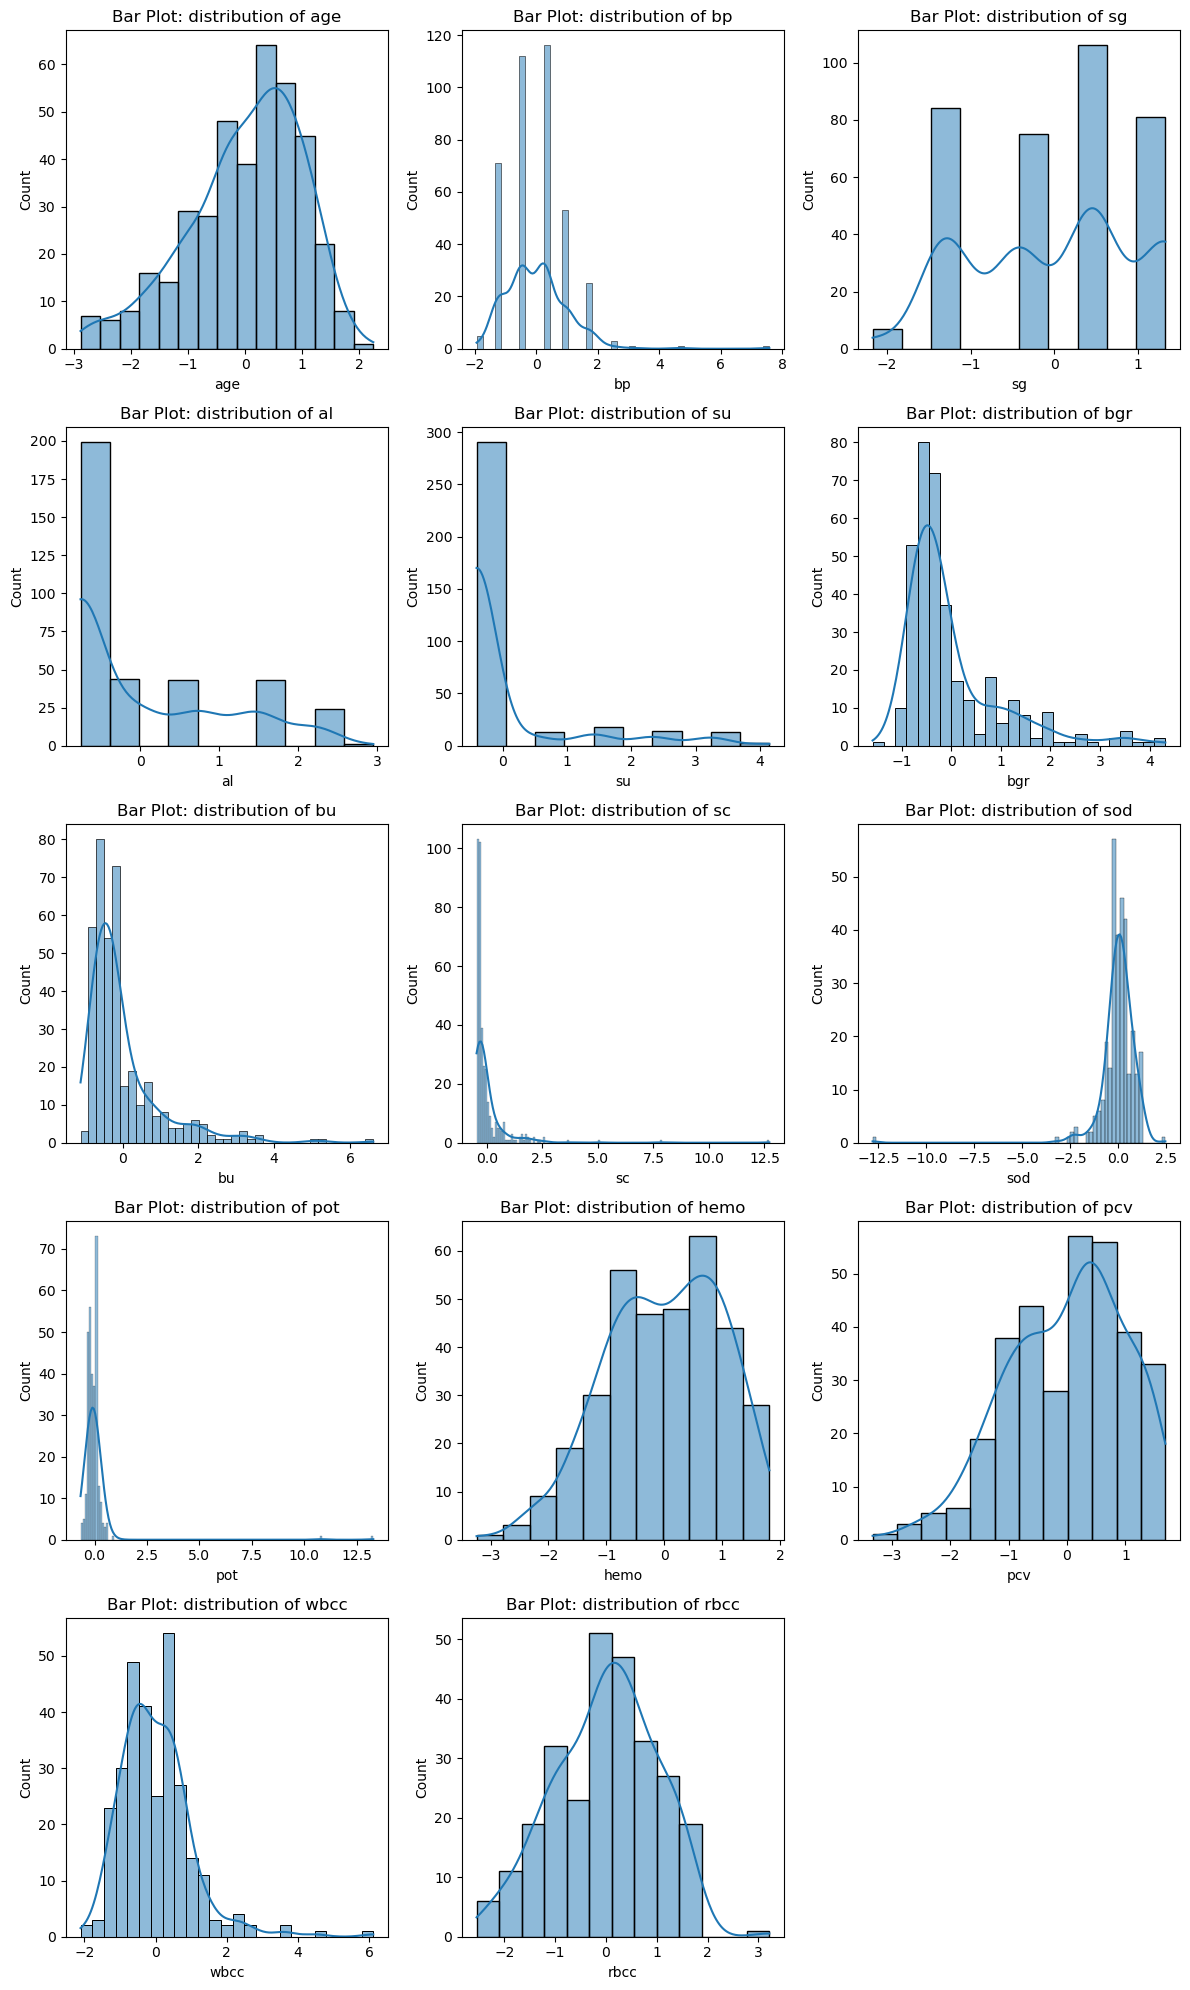
\includegraphics{assignment6111_files/figure-pdf/cell-17-output-1.png}

\begin{enumerate}
\def\labelenumi{\arabic{enumi}.}
\setcounter{enumi}{3}
\tightlist
\item
  Association Between Variables
\end{enumerate}

\begin{itemize}
\tightlist
\item
  We use two methods to analyze the association between these variables.
  Firstly, we use heat map to analyze the association between all
  numerical datas. After that, we use histogram to analyze the
  association between all categorical variables.
\end{itemize}

\begin{Shaded}
\begin{Highlighting}[]
\NormalTok{plt.figure(figsize}\OperatorTok{=}\NormalTok{(}\DecValTok{15}\NormalTok{, }\DecValTok{10}\NormalTok{))}
\NormalTok{sns.heatmap(X\_reg[numerical].corr(), annot}\OperatorTok{=}\VariableTok{True}\NormalTok{,cmap}\OperatorTok{=}\StringTok{\textquotesingle{}viridis\textquotesingle{}}\NormalTok{)}
\end{Highlighting}
\end{Shaded}

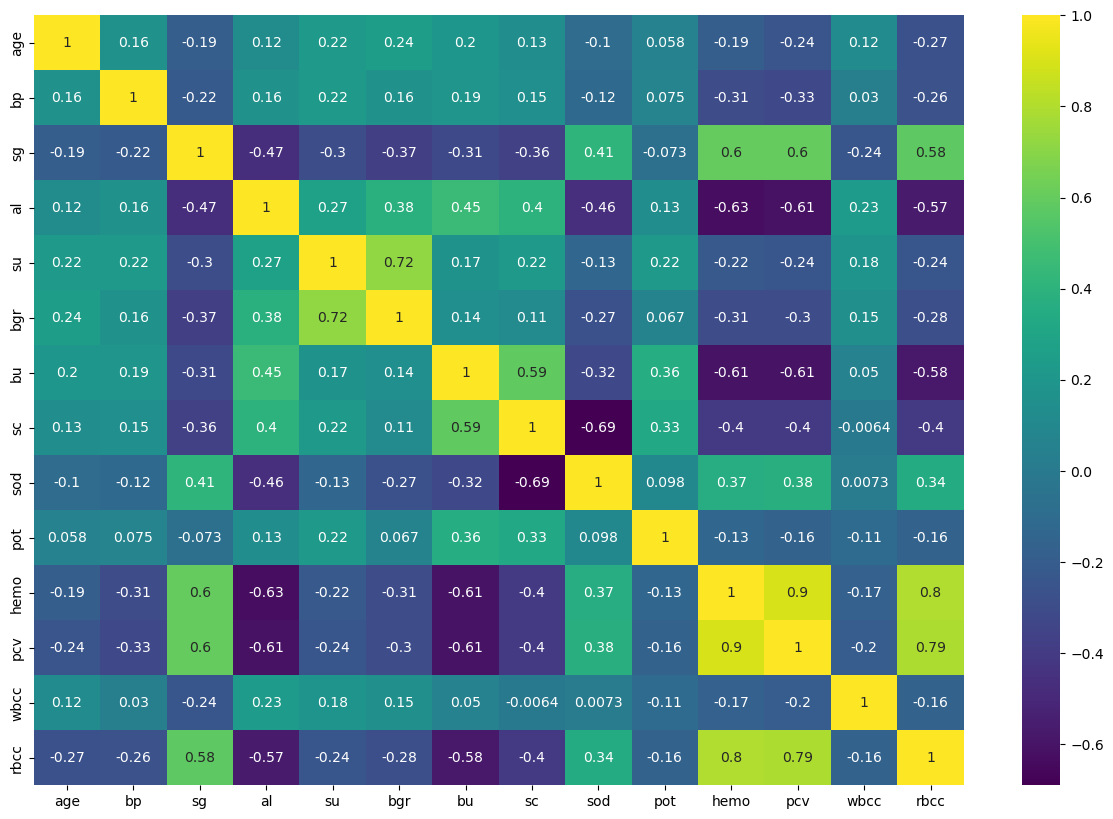
\includegraphics{assignment6111_files/figure-pdf/cell-18-output-1.png}

\begin{itemize}
\tightlist
\item
  According to the heatmap, lighter colour represent a higher
  association and vise versa. For example, pcv, hemo, and rbcc has high
  association with each other. However, the heatmap shows that all
  numerical variables have a less association overall because most of
  them are under 0.5.
\end{itemize}

\begin{Shaded}
\begin{Highlighting}[]
\ImportTok{import}\NormalTok{ matplotlib.pyplot }\ImportTok{as}\NormalTok{ plt}
\ImportTok{import}\NormalTok{ seaborn }\ImportTok{as}\NormalTok{ sns}

\NormalTok{categorical}\OperatorTok{=}\NormalTok{X\_reg.select\_dtypes(include}\OperatorTok{=}\StringTok{\textquotesingle{}int8\textquotesingle{}}\NormalTok{).columns}

\NormalTok{n\_rows }\OperatorTok{=} \DecValTok{3}
\NormalTok{n\_cols }\OperatorTok{=} \DecValTok{4}

\NormalTok{fig, axes }\OperatorTok{=}\NormalTok{ plt.subplots(n\_rows, n\_cols, figsize}\OperatorTok{=}\NormalTok{(n\_cols }\OperatorTok{*} \DecValTok{4}\NormalTok{, n\_rows }\OperatorTok{*} \DecValTok{4}\NormalTok{))}
\NormalTok{axes\_flat }\OperatorTok{=}\NormalTok{ axes.flatten()}

\ControlFlowTok{for}\NormalTok{ i, term }\KeywordTok{in} \BuiltInTok{enumerate}\NormalTok{(categorical):}
\NormalTok{    sns.countplot(}
\NormalTok{        data}\OperatorTok{=}\NormalTok{X\_reg,}
\NormalTok{        x}\OperatorTok{=}\NormalTok{term,}
\NormalTok{        color}\OperatorTok{=}\StringTok{"purple"}\NormalTok{,}
\NormalTok{        ax}\OperatorTok{=}\NormalTok{axes\_flat[i] }
\NormalTok{    )}
\NormalTok{    axes\_flat[i].set\_xlabel(term)}
\NormalTok{    axes\_flat[i].set\_ylabel(}\StringTok{"Count"}\NormalTok{)}
\NormalTok{    axes\_flat[i].set\_title(}\StringTok{"Bar Plot: distribution of "} \OperatorTok{+}\NormalTok{ term)}

\ControlFlowTok{for}\NormalTok{ j }\KeywordTok{in} \BuiltInTok{range}\NormalTok{(i}\OperatorTok{+}\DecValTok{1}\NormalTok{, n\_rows}\OperatorTok{*}\NormalTok{n\_cols):}
\NormalTok{    fig.delaxes(axes\_flat[j])}

\NormalTok{plt.tight\_layout()}

\NormalTok{plt.show()}
\end{Highlighting}
\end{Shaded}

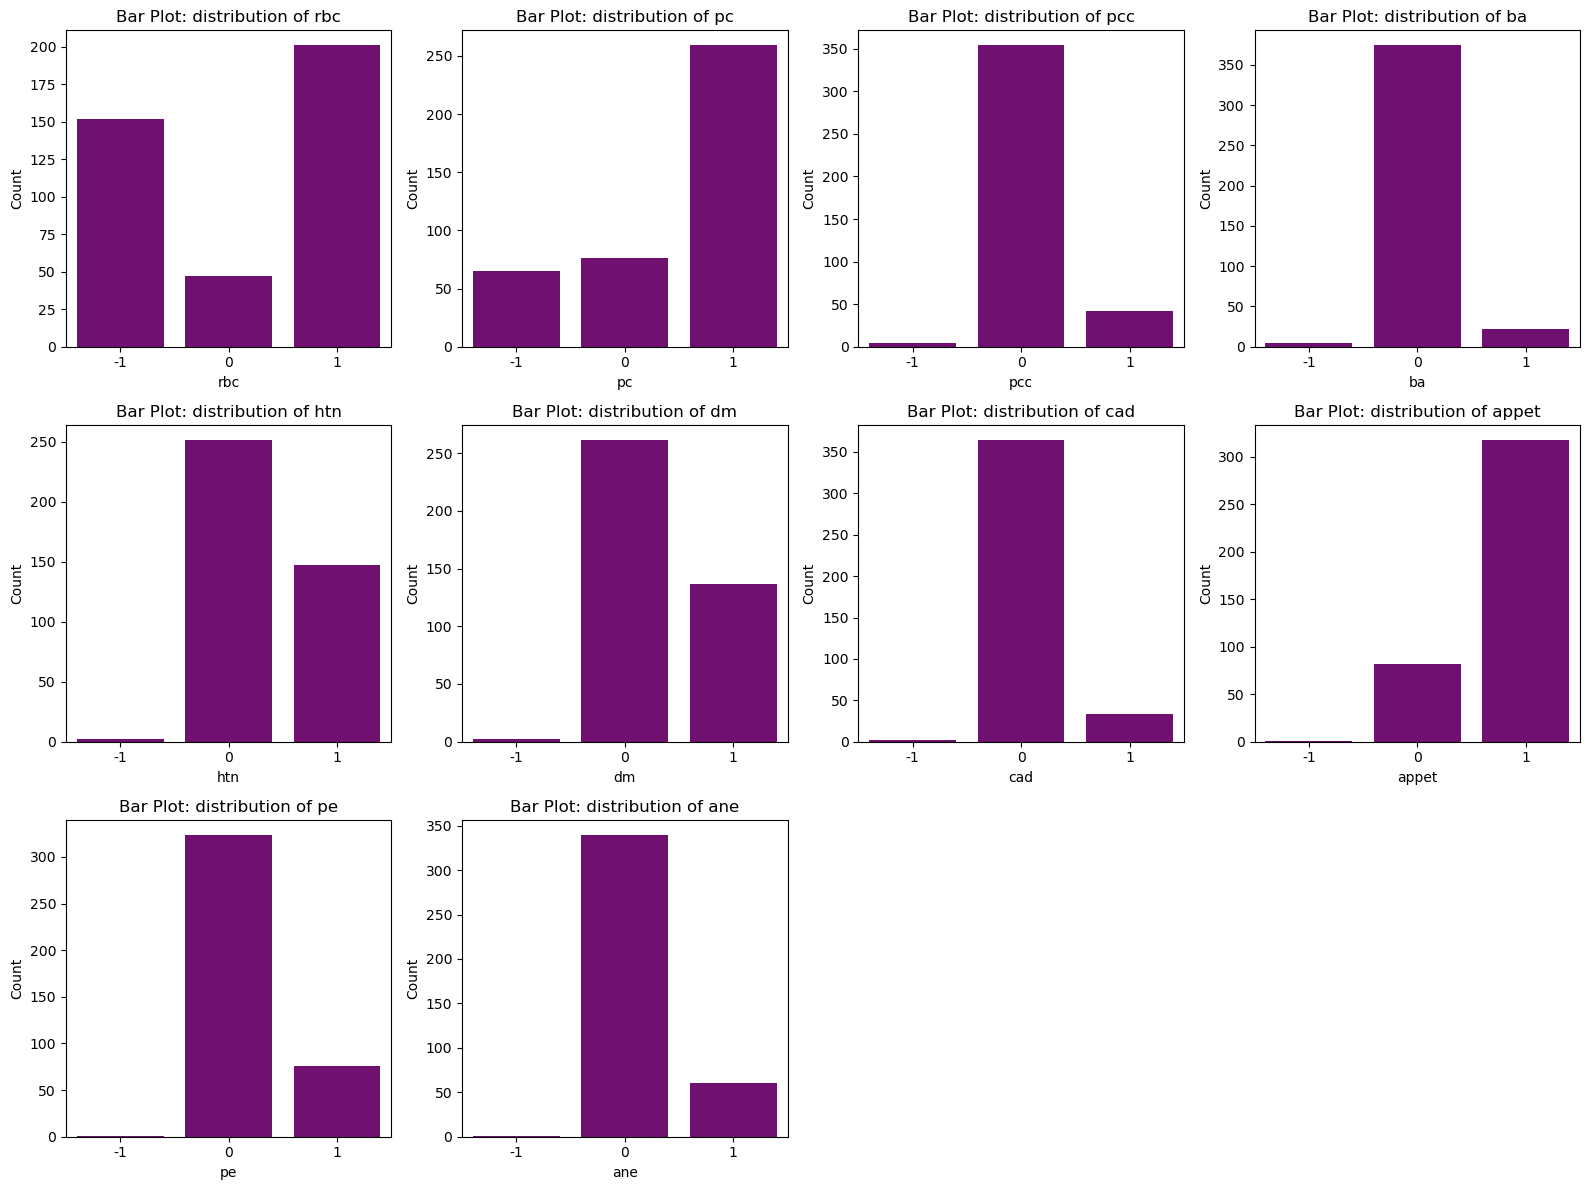
\includegraphics{assignment6111_files/figure-pdf/cell-19-output-1.png}

term- From histograms, for implication of these categorical variables
for feature selection, if the -1 term appears more then 50 times, we
could conclude that there are too many NA in this varibale, we need to
drop this term during feature selection, such as ``rbc'' and ``pc''. The
histogram of rbc has many missing values so it may not be significant
for feature selection.

\begin{enumerate}
\def\labelenumi{\arabic{enumi}.}
\setcounter{enumi}{4}
\tightlist
\item
  Missing Value Analysis and Handling
\end{enumerate}

\begin{Shaded}
\begin{Highlighting}[]
\NormalTok{X.isna().}\BuiltInTok{sum}\NormalTok{()}
\end{Highlighting}
\end{Shaded}

\begin{verbatim}
age        9
bp        12
sg        47
al        46
su        49
rbc      152
pc        65
pcc        4
ba         4
bgr       44
bu        19
sc        17
sod       87
pot       88
hemo      52
pcv       71
wbcc     106
rbcc     131
htn        2
dm         2
cad        2
appet      1
pe         1
ane        1
dtype: int64
\end{verbatim}

\begin{itemize}
\tightlist
\item
  From above, we can see there are missing values everywhere. We decided
  to remove variables that have more than 50 missing values because too
  many missing values result in an inaccurate analysis.
\end{itemize}

\begin{Shaded}
\begin{Highlighting}[]
\NormalTok{m\_value }\OperatorTok{=}\NormalTok{ X\_reg.isna().}\BuiltInTok{sum}\NormalTok{()}

\NormalTok{m\_value\_df }\OperatorTok{=}\NormalTok{ pd.DataFrame(m\_value, columns}\OperatorTok{=}\NormalTok{[}\StringTok{"missing values"}\NormalTok{])}
\NormalTok{bigm }\OperatorTok{=}\NormalTok{ m\_value\_df[m\_value\_df[}\StringTok{"missing values"}\NormalTok{]}\OperatorTok{\textgreater{}}\DecValTok{50}\NormalTok{].index}
\NormalTok{bigm}
\end{Highlighting}
\end{Shaded}

\begin{verbatim}
Index(['sod', 'pot', 'hemo', 'pcv', 'wbcc', 'rbcc'], dtype='object')
\end{verbatim}

\begin{Shaded}
\begin{Highlighting}[]
\ImportTok{from}\NormalTok{ sklearn.impute }\ImportTok{import}\NormalTok{ KNNImputer}

\NormalTok{X\_new }\OperatorTok{=}\NormalTok{ X\_reg.drop(columns}\OperatorTok{=}\NormalTok{bigm)}
\NormalTok{imputer }\OperatorTok{=}\NormalTok{ KNNImputer(n\_neighbors}\OperatorTok{=}\DecValTok{5}\NormalTok{)}
\NormalTok{X\_new }\OperatorTok{=}\NormalTok{ pd.DataFrame(imputer.fit\_transform(X\_new), columns}\OperatorTok{=}\NormalTok{X\_new.columns)}
\NormalTok{X\_new.isna().}\BuiltInTok{sum}\NormalTok{()}
\end{Highlighting}
\end{Shaded}

\begin{verbatim}
age      0
bp       0
sg       0
al       0
su       0
rbc      0
pc       0
pcc      0
ba       0
bgr      0
bu       0
sc       0
htn      0
dm       0
cad      0
appet    0
pe       0
ane      0
dtype: int64
\end{verbatim}

\begin{enumerate}
\def\labelenumi{\arabic{enumi}.}
\setcounter{enumi}{5}
\tightlist
\item
  Outlier Analysis:
\end{enumerate}

\begin{Shaded}
\begin{Highlighting}[]
\NormalTok{new\_columns }\OperatorTok{=}\NormalTok{[}\StringTok{\textquotesingle{}age\textquotesingle{}}\NormalTok{, }\StringTok{\textquotesingle{}bp\textquotesingle{}}\NormalTok{, }\StringTok{\textquotesingle{}bgr\textquotesingle{}}\NormalTok{, }\StringTok{\textquotesingle{}bu\textquotesingle{}}\NormalTok{, }\StringTok{\textquotesingle{}sc\textquotesingle{}}\NormalTok{]}

\NormalTok{boxplot\_data }\OperatorTok{=}\NormalTok{ X\_new[new\_columns]}

\NormalTok{plt.figure(figsize}\OperatorTok{=}\NormalTok{(}\DecValTok{10}\NormalTok{, }\DecValTok{6}\NormalTok{)) }
\NormalTok{boxplot\_data.boxplot()}
\NormalTok{plt.title(}\StringTok{\textquotesingle{}Boxplot of Selected Variables\textquotesingle{}}\NormalTok{)}
\NormalTok{plt.xlabel(}\StringTok{\textquotesingle{}Variables\textquotesingle{}}\NormalTok{)}
\NormalTok{plt.ylabel(}\StringTok{\textquotesingle{}Values\textquotesingle{}}\NormalTok{)}
\NormalTok{plt.xticks(rotation}\OperatorTok{=}\DecValTok{45}\NormalTok{)  }
\NormalTok{plt.grid(axis}\OperatorTok{=}\StringTok{\textquotesingle{}y\textquotesingle{}}\NormalTok{)  }
\NormalTok{plt.show()}
\end{Highlighting}
\end{Shaded}

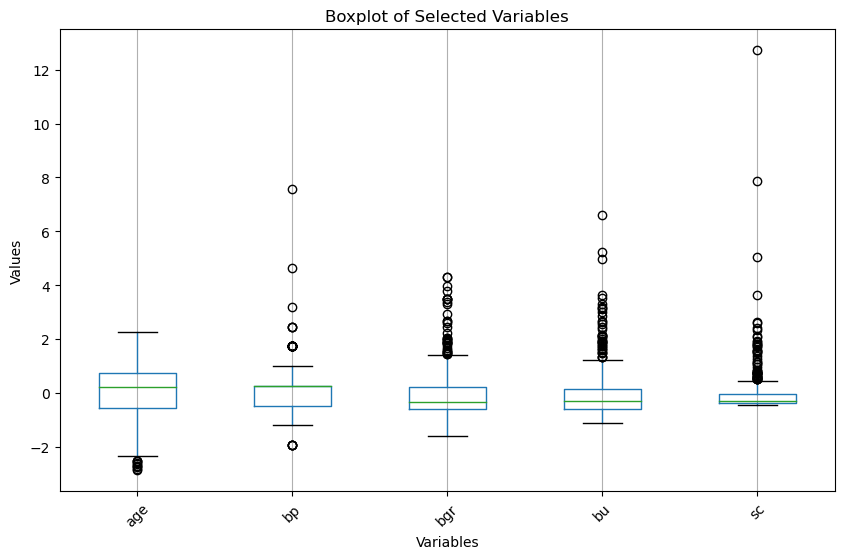
\includegraphics{assignment6111_files/figure-pdf/cell-23-output-1.png}

Looking at the box plot for all the remaining numerical variables, we
see that all variables have outliers, but ``bp'' and ``sc'' variables
have outlier relatively large outlier, especially for ``sc'', so we want
to delelte the entire row for these outlier with value greater thenm 6.
In this case our data would give us better estimation.

\begin{Shaded}
\begin{Highlighting}[]
\NormalTok{X\_new\_dummy }\OperatorTok{=}\NormalTok{ pd.DataFrame(X\_new, columns}\OperatorTok{=}\NormalTok{[}\StringTok{\textquotesingle{}age\textquotesingle{}}\NormalTok{, }\StringTok{\textquotesingle{}bp\textquotesingle{}}\NormalTok{, }\StringTok{\textquotesingle{}sg\textquotesingle{}}\NormalTok{, }\StringTok{\textquotesingle{}al\textquotesingle{}}\NormalTok{, }\StringTok{\textquotesingle{}su\textquotesingle{}}\NormalTok{]) }
\NormalTok{X\_new\_dummy }\OperatorTok{=}\NormalTok{ X\_new\_dummy[(X\_new\_dummy }\OperatorTok{\textless{}=} \DecValTok{6}\NormalTok{).}\BuiltInTok{all}\NormalTok{(axis}\OperatorTok{=}\DecValTok{1}\NormalTok{)] }
\NormalTok{X\_new\_dummy.describe}
\end{Highlighting}
\end{Shaded}

\begin{verbatim}
<bound method NDFrame.describe of           age        bp        sg        al        su
0   -0.203139  0.258373  0.454071 -0.012548 -0.410106
1   -2.594124 -1.936857  0.454071  2.208413 -0.410106
2    0.613295  0.258373 -1.297699  0.727772  2.323069
3   -0.203139 -0.473370 -2.173584  2.208413 -0.410106
4   -0.028189  0.258373 -1.297699  0.727772 -0.410106
..        ...       ...       ...       ...       ...
395  0.205078  0.258373  0.454071 -0.752868 -0.410106
396 -0.553039 -0.473370  1.329955 -0.752868 -0.410106
397 -2.302541  0.258373  0.454071 -0.752868 -0.410106
398 -2.010957 -1.205114  1.329955 -0.752868 -0.410106
399  0.380028  0.258373  1.329955 -0.752868 -0.410106

[399 rows x 5 columns]>
\end{verbatim}

Here we can clearly check the outlier has been removed. we also so the
same index change in y

\begin{Shaded}
\begin{Highlighting}[]
\NormalTok{outlier\_indices }\OperatorTok{=}\NormalTok{ X\_new.index[X\_new.}\BuiltInTok{apply}\NormalTok{(}\KeywordTok{lambda}\NormalTok{ x: (x }\OperatorTok{\textgreater{}} \DecValTok{6}\NormalTok{).}\BuiltInTok{any}\NormalTok{(), axis}\OperatorTok{=}\DecValTok{1}\NormalTok{)].tolist() }
\NormalTok{outlier\_indices}
\NormalTok{X\_new\_dummy\_dropped }\OperatorTok{=}\NormalTok{ X\_new.drop(index}\OperatorTok{=}\NormalTok{outlier\_indices)}
\NormalTok{y\_new}\OperatorTok{=}\NormalTok{y.drop(index}\OperatorTok{=}\NormalTok{outlier\_indices)}
\end{Highlighting}
\end{Shaded}

\begin{Shaded}
\begin{Highlighting}[]
\NormalTok{y\_new[}\StringTok{\textquotesingle{}class\textquotesingle{}}\NormalTok{] }\OperatorTok{=}\NormalTok{ y\_new[}\StringTok{"class"}\NormalTok{].astype(}\StringTok{\textquotesingle{}category\textquotesingle{}}\NormalTok{).cat.codes}
\NormalTok{y\_new}
\end{Highlighting}
\end{Shaded}

\begin{longtable}[]{@{}ll@{}}
\toprule\noalign{}
& class \\
\midrule\noalign{}
\endhead
\bottomrule\noalign{}
\endlastfoot
0 & 0 \\
1 & 0 \\
2 & 0 \\
3 & 0 \\
4 & 0 \\
... & ... \\
395 & 1 \\
396 & 1 \\
397 & 1 \\
398 & 1 \\
399 & 1 \\
\end{longtable}

\begin{enumerate}
\def\labelenumi{\arabic{enumi}.}
\setcounter{enumi}{6}
\tightlist
\item
  Sub-group Analysis
\end{enumerate}

\begin{Shaded}
\begin{Highlighting}[]
\CommentTok{\#\#K{-}means}
\ImportTok{from}\NormalTok{ sklearn.preprocessing }\ImportTok{import}\NormalTok{ scale}
\ImportTok{from}\NormalTok{ sklearn.decomposition }\ImportTok{import}\NormalTok{ PCA, TruncatedSVD}
\ImportTok{from}\NormalTok{ sklearn.cluster }\ImportTok{import}\NormalTok{ KMeans}
\ImportTok{from}\NormalTok{ scipy.cluster }\ImportTok{import}\NormalTok{ hierarchy}
\ImportTok{from}\NormalTok{ sklearn.cluster }\ImportTok{import}\NormalTok{ AgglomerativeClustering}
\ImportTok{from}\NormalTok{ sklearn.metrics }\ImportTok{import}\NormalTok{ silhouette\_samples, silhouette\_score}
\ImportTok{from}\NormalTok{ sklearn.metrics.cluster }\ImportTok{import}\NormalTok{ rand\_score}
\ImportTok{from}\NormalTok{ sklearn.preprocessing }\ImportTok{import}\NormalTok{ StandardScaler}
\ImportTok{from}\NormalTok{ sklearn.metrics }\ImportTok{import}\NormalTok{ adjusted\_rand\_score}
\ImportTok{from}\NormalTok{ sklearn.decomposition }\ImportTok{import}\NormalTok{ PCA, TruncatedSVD, FactorAnalysis}
\ImportTok{import}\NormalTok{ matplotlib.pyplot }\ImportTok{as}\NormalTok{ plt}
\ImportTok{from}\NormalTok{ sklearn.metrics }\ImportTok{import}\NormalTok{ silhouette\_score, silhouette\_samples}
\ImportTok{from}\NormalTok{ matplotlib }\ImportTok{import}\NormalTok{ cm  }\CommentTok{\# Import colormap directly from matplotlib.cm}
\end{Highlighting}
\end{Shaded}

\begin{Shaded}
\begin{Highlighting}[]
\NormalTok{y[}\StringTok{\textquotesingle{}class\textquotesingle{}}\NormalTok{] }\OperatorTok{=}\NormalTok{ y[}\StringTok{"class"}\NormalTok{].astype(}\StringTok{\textquotesingle{}category\textquotesingle{}}\NormalTok{).cat.codes}

\NormalTok{km1 }\OperatorTok{=}\NormalTok{ KMeans(n\_clusters}\OperatorTok{=}\DecValTok{2}\NormalTok{, n\_init}\OperatorTok{=}\DecValTok{20}\NormalTok{, random\_state}\OperatorTok{=}\DecValTok{0}\NormalTok{)}
\NormalTok{km1.fit(X\_new\_dummy\_dropped)}
\NormalTok{km1.labels\_}
\end{Highlighting}
\end{Shaded}

\begin{verbatim}
/var/folders/8d/rl260sm16jzgyscznl23d0z80000gn/T/ipykernel_57231/1292506993.py:1: SettingWithCopyWarning: 
A value is trying to be set on a copy of a slice from a DataFrame.
Try using .loc[row_indexer,col_indexer] = value instead

See the caveats in the documentation: https://pandas.pydata.org/pandas-docs/stable/user_guide/indexing.html#returning-a-view-versus-a-copy
  y['class'] = y["class"].astype('category').cat.codes
\end{verbatim}

\begin{verbatim}
array([0, 0, 1, 1, 0, 1, 1, 1, 1, 1, 1, 1, 1, 1, 1, 1, 0, 1, 1, 0, 1, 1,
       0, 1, 0, 1, 1, 1, 1, 1, 1, 1, 1, 1, 1, 0, 1, 1, 1, 1, 0, 1, 1, 1,
       1, 0, 0, 0, 1, 1, 1, 0, 1, 1, 1, 1, 1, 1, 1, 1, 0, 0, 1, 0, 1, 1,
       1, 1, 1, 1, 1, 1, 1, 0, 1, 1, 1, 1, 1, 1, 1, 0, 1, 1, 1, 1, 1, 0,
       1, 1, 1, 1, 1, 1, 1, 1, 1, 1, 1, 0, 1, 1, 0, 1, 1, 0, 1, 0, 1, 0,
       1, 0, 0, 0, 0, 1, 0, 1, 1, 1, 1, 1, 1, 1, 1, 1, 0, 1, 0, 1, 1, 1,
       1, 1, 1, 1, 1, 1, 1, 1, 1, 1, 1, 1, 1, 0, 0, 1, 0, 1, 1, 0, 1, 0,
       1, 1, 1, 1, 1, 1, 0, 1, 0, 0, 1, 1, 1, 1, 1, 0, 1, 1, 1, 1, 1, 1,
       1, 0, 0, 0, 1, 0, 0, 0, 0, 1, 0, 1, 0, 1, 1, 1, 1, 1, 1, 0, 1, 1,
       1, 1, 1, 1, 1, 1, 1, 0, 1, 0, 1, 1, 1, 0, 0, 1, 0, 1, 0, 1, 1, 1,
       0, 1, 1, 0, 1, 1, 1, 1, 1, 0, 0, 1, 1, 1, 1, 0, 1, 1, 1, 1, 1, 1,
       1, 0, 1, 1, 0, 0, 0, 0, 0, 0, 0, 0, 0, 0, 0, 0, 0, 0, 0, 0, 0, 0,
       0, 0, 0, 0, 0, 0, 0, 0, 0, 0, 0, 0, 0, 0, 0, 0, 0, 0, 0, 0, 0, 0,
       0, 0, 0, 0, 0, 0, 0, 0, 0, 0, 0, 0, 0, 0, 0, 0, 0, 0, 0, 0, 0, 0,
       0, 0, 0, 0, 0, 0, 0, 0, 0, 0, 0, 0, 0, 0, 0, 0, 0, 0, 0, 0, 0, 0,
       0, 0, 0, 0, 0, 0, 0, 0, 0, 0, 0, 0, 0, 0, 0, 0, 0, 0, 0, 0, 0, 0,
       0, 0, 0, 0, 0, 0, 0, 0, 0, 0, 0, 0, 0, 0, 0, 0, 0, 0, 0, 0, 0, 0,
       0, 0, 0, 0, 0, 0, 0, 0, 0, 0, 0, 0, 0, 0, 0, 0, 0, 0, 0, 0, 0, 0],
      dtype=int32)
\end{verbatim}

\begin{Shaded}
\begin{Highlighting}[]
\NormalTok{range\_n\_clusters }\OperatorTok{=}\NormalTok{ [}\DecValTok{2}\NormalTok{, }\DecValTok{3}\NormalTok{, }\DecValTok{4}\NormalTok{, }\DecValTok{5}\NormalTok{, }\DecValTok{6}\NormalTok{]}
\ControlFlowTok{for}\NormalTok{ n\_clusters }\KeywordTok{in}\NormalTok{ range\_n\_clusters:}
\NormalTok{    km }\OperatorTok{=}\NormalTok{ KMeans(n\_clusters}\OperatorTok{=}\NormalTok{n\_clusters, n\_init}\OperatorTok{=}\DecValTok{20}\NormalTok{, random\_state}\OperatorTok{=}\DecValTok{0}\NormalTok{)}
\NormalTok{    labels }\OperatorTok{=}\NormalTok{ km.fit\_predict(X\_new\_dummy\_dropped)}
    
\NormalTok{    silhouette\_avg }\OperatorTok{=}\NormalTok{ silhouette\_score(X\_new\_dummy\_dropped, labels)}
\NormalTok{    sample\_silhouette\_values }\OperatorTok{=}\NormalTok{ silhouette\_samples(X\_new\_dummy\_dropped, labels)}
\NormalTok{    fig, ax1 }\OperatorTok{=}\NormalTok{ plt.subplots(}\DecValTok{1}\NormalTok{, }\DecValTok{1}\NormalTok{)}
\NormalTok{    fig.set\_size\_inches(}\DecValTok{18}\NormalTok{, }\DecValTok{7}\NormalTok{)}
\NormalTok{    ax1.set\_xlim([}\OperatorTok{{-}}\FloatTok{0.3}\NormalTok{, }\DecValTok{1}\NormalTok{])}

\NormalTok{    y\_lower }\OperatorTok{=} \DecValTok{10}
    
    \ControlFlowTok{for}\NormalTok{ i }\KeywordTok{in} \BuiltInTok{range}\NormalTok{(n\_clusters):}
\NormalTok{        ith\_cluster\_silhouette\_values }\OperatorTok{=}\NormalTok{ sample\_silhouette\_values[labels }\OperatorTok{==}\NormalTok{ i]}
\NormalTok{        ith\_cluster\_silhouette\_values.sort()}

\NormalTok{        size\_cluster\_i }\OperatorTok{=}\NormalTok{ ith\_cluster\_silhouette\_values.shape[}\DecValTok{0}\NormalTok{]}
\NormalTok{        y\_upper }\OperatorTok{=}\NormalTok{ y\_lower }\OperatorTok{+}\NormalTok{ size\_cluster\_i}

\NormalTok{        color }\OperatorTok{=}\NormalTok{ cm.nipy\_spectral(}\BuiltInTok{float}\NormalTok{(i) }\OperatorTok{/}\NormalTok{ n\_clusters)}
\NormalTok{        ax1.fill\_betweenx(}
\NormalTok{            y}\OperatorTok{=}\NormalTok{np.arange(y\_lower, y\_upper),}
\NormalTok{            x1}\OperatorTok{=}\DecValTok{0}\NormalTok{,}
\NormalTok{            x2}\OperatorTok{=}\NormalTok{ith\_cluster\_silhouette\_values,}
\NormalTok{            facecolor}\OperatorTok{=}\NormalTok{color,}
\NormalTok{            edgecolor}\OperatorTok{=}\NormalTok{color,}
\NormalTok{            alpha}\OperatorTok{=}\FloatTok{0.7}\NormalTok{,}
\NormalTok{        )}

\NormalTok{        ax1.text(}\OperatorTok{{-}}\FloatTok{0.05}\NormalTok{, y\_lower }\OperatorTok{+} \FloatTok{0.5} \OperatorTok{*}\NormalTok{ size\_cluster\_i, }\BuiltInTok{str}\NormalTok{(i))}

\NormalTok{        y\_lower }\OperatorTok{=}\NormalTok{ y\_upper }\OperatorTok{+} \DecValTok{10}  

\NormalTok{    ax1.set\_title(}\StringTok{"The silhouette plot for various clusters"}\NormalTok{)}
\NormalTok{    ax1.set\_xlabel(}\StringTok{"The silhouette coefficient values"}\NormalTok{)}
\NormalTok{    ax1.set\_ylabel(}\StringTok{"Cluster label"}\NormalTok{)}

\NormalTok{    ax1.axvline(x}\OperatorTok{=}\NormalTok{silhouette\_avg, color}\OperatorTok{=}\StringTok{"red"}\NormalTok{, linestyle}\OperatorTok{=}\StringTok{"{-}{-}"}\NormalTok{)}
\NormalTok{    plt.title(}
        \StringTok{"Silhouette analysis for KMeans clustering on sample data with n\_clusters = }\SpecialCharTok{\%d}\StringTok{"}
        \OperatorTok{\%}\NormalTok{ n\_clusters,}
\NormalTok{        fontsize}\OperatorTok{=}\DecValTok{14}\NormalTok{,}
\NormalTok{        fontweight}\OperatorTok{=}\StringTok{"bold"}\NormalTok{,}
\NormalTok{    )}

\NormalTok{plt.show()}
\end{Highlighting}
\end{Shaded}

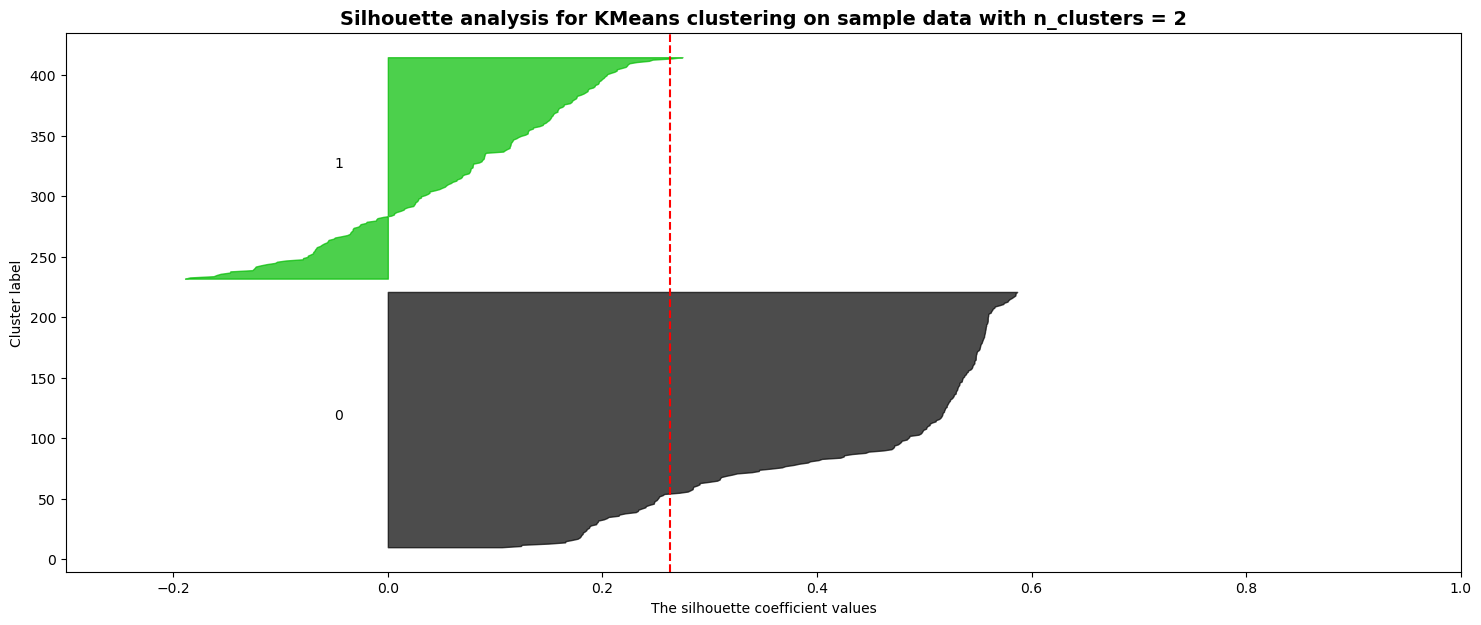
\includegraphics{assignment6111_files/figure-pdf/cell-29-output-1.png}

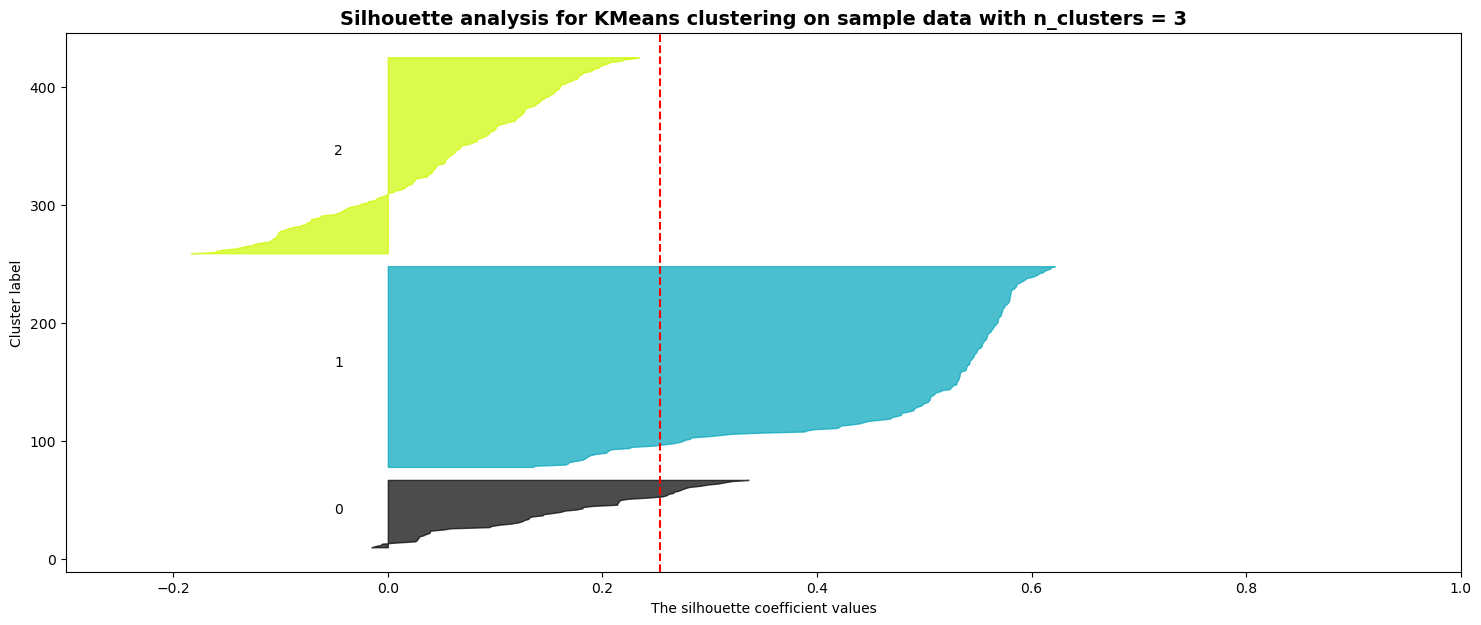
\includegraphics{assignment6111_files/figure-pdf/cell-29-output-2.png}

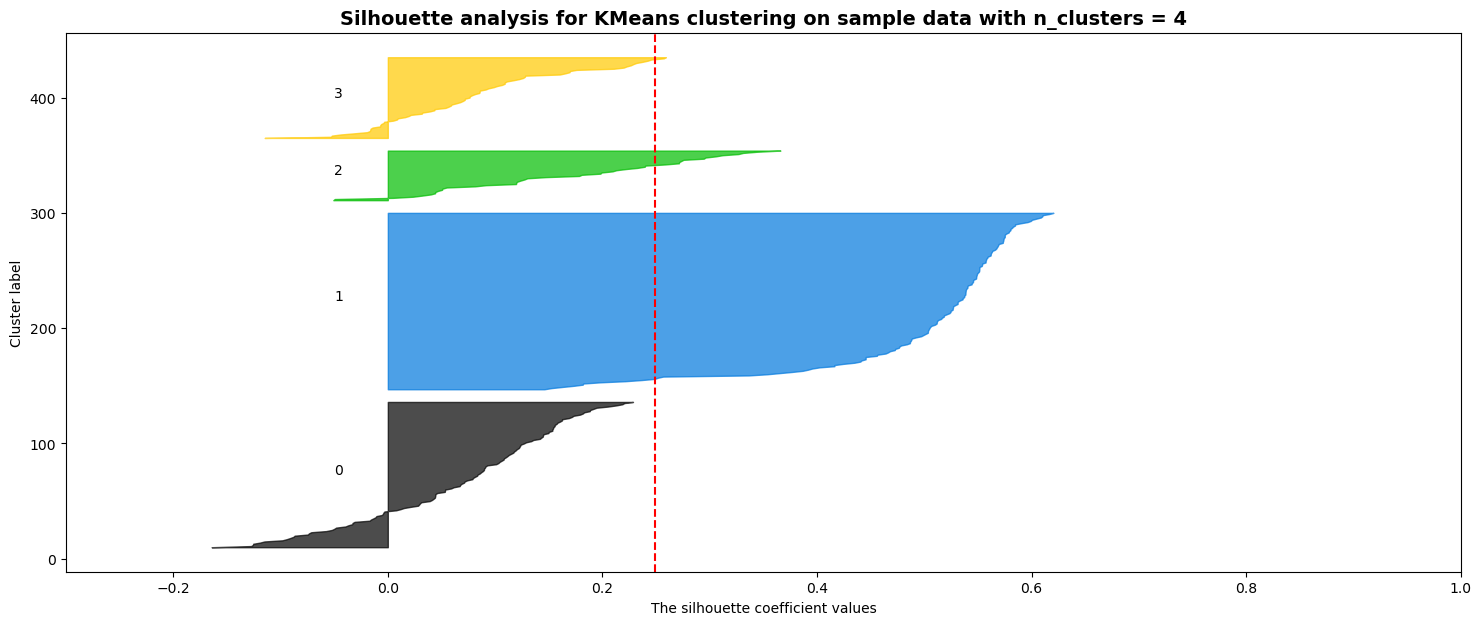
\includegraphics{assignment6111_files/figure-pdf/cell-29-output-3.png}

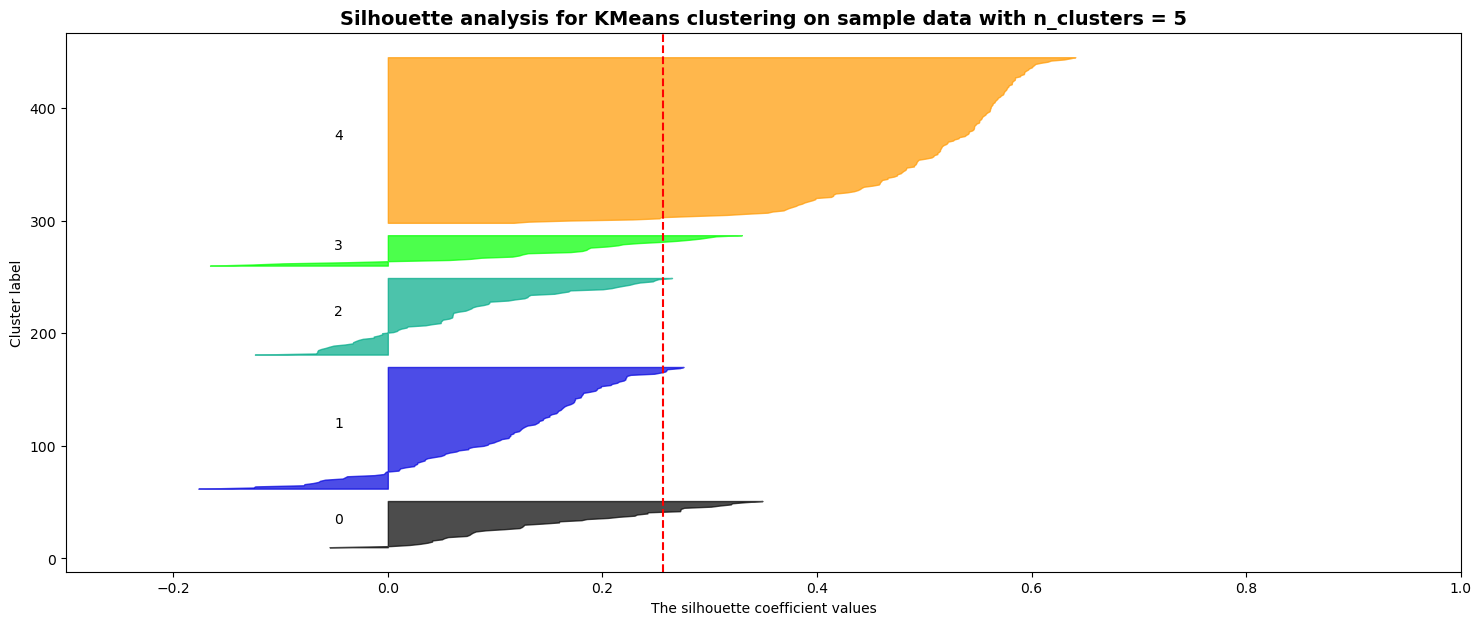
\includegraphics{assignment6111_files/figure-pdf/cell-29-output-4.png}

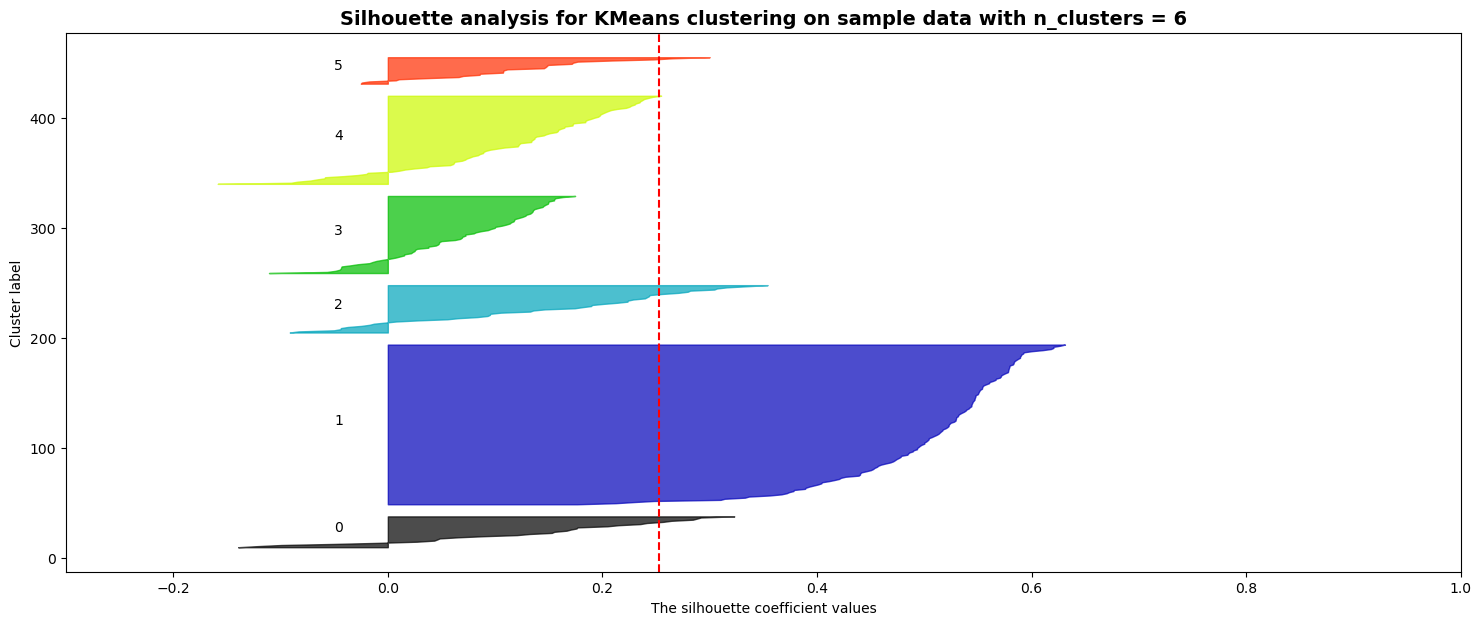
\includegraphics{assignment6111_files/figure-pdf/cell-29-output-5.png}

\begin{Shaded}
\begin{Highlighting}[]
\CommentTok{\#use k=2}
\NormalTok{kmeans }\OperatorTok{=}\NormalTok{ KMeans(n\_clusters}\OperatorTok{=}\DecValTok{2}\NormalTok{, n\_init}\OperatorTok{=}\DecValTok{20}\NormalTok{, random\_state}\OperatorTok{=}\DecValTok{0}\NormalTok{)}
\NormalTok{labels }\OperatorTok{=}\NormalTok{ kmeans.fit\_predict(X\_new\_dummy\_dropped)}
\NormalTok{labels}
\end{Highlighting}
\end{Shaded}

\begin{verbatim}
array([0, 0, 1, 1, 0, 1, 1, 1, 1, 1, 1, 1, 1, 1, 1, 1, 0, 1, 1, 0, 1, 1,
       0, 1, 0, 1, 1, 1, 1, 1, 1, 1, 1, 1, 1, 0, 1, 1, 1, 1, 0, 1, 1, 1,
       1, 0, 0, 0, 1, 1, 1, 0, 1, 1, 1, 1, 1, 1, 1, 1, 0, 0, 1, 0, 1, 1,
       1, 1, 1, 1, 1, 1, 1, 0, 1, 1, 1, 1, 1, 1, 1, 0, 1, 1, 1, 1, 1, 0,
       1, 1, 1, 1, 1, 1, 1, 1, 1, 1, 1, 0, 1, 1, 0, 1, 1, 0, 1, 0, 1, 0,
       1, 0, 0, 0, 0, 1, 0, 1, 1, 1, 1, 1, 1, 1, 1, 1, 0, 1, 0, 1, 1, 1,
       1, 1, 1, 1, 1, 1, 1, 1, 1, 1, 1, 1, 1, 0, 0, 1, 0, 1, 1, 0, 1, 0,
       1, 1, 1, 1, 1, 1, 0, 1, 0, 0, 1, 1, 1, 1, 1, 0, 1, 1, 1, 1, 1, 1,
       1, 0, 0, 0, 1, 0, 0, 0, 0, 1, 0, 1, 0, 1, 1, 1, 1, 1, 1, 0, 1, 1,
       1, 1, 1, 1, 1, 1, 1, 0, 1, 0, 1, 1, 1, 0, 0, 1, 0, 1, 0, 1, 1, 1,
       0, 1, 1, 0, 1, 1, 1, 1, 1, 0, 0, 1, 1, 1, 1, 0, 1, 1, 1, 1, 1, 1,
       1, 0, 1, 1, 0, 0, 0, 0, 0, 0, 0, 0, 0, 0, 0, 0, 0, 0, 0, 0, 0, 0,
       0, 0, 0, 0, 0, 0, 0, 0, 0, 0, 0, 0, 0, 0, 0, 0, 0, 0, 0, 0, 0, 0,
       0, 0, 0, 0, 0, 0, 0, 0, 0, 0, 0, 0, 0, 0, 0, 0, 0, 0, 0, 0, 0, 0,
       0, 0, 0, 0, 0, 0, 0, 0, 0, 0, 0, 0, 0, 0, 0, 0, 0, 0, 0, 0, 0, 0,
       0, 0, 0, 0, 0, 0, 0, 0, 0, 0, 0, 0, 0, 0, 0, 0, 0, 0, 0, 0, 0, 0,
       0, 0, 0, 0, 0, 0, 0, 0, 0, 0, 0, 0, 0, 0, 0, 0, 0, 0, 0, 0, 0, 0,
       0, 0, 0, 0, 0, 0, 0, 0, 0, 0, 0, 0, 0, 0, 0, 0, 0, 0, 0, 0, 0, 0],
      dtype=int32)
\end{verbatim}

\begin{Shaded}
\begin{Highlighting}[]
\NormalTok{pca\_X }\OperatorTok{=}\NormalTok{ PCA()}
\NormalTok{X }\OperatorTok{=}\NormalTok{ pd.DataFrame(X\_new\_dummy\_dropped, X\_new\_dummy\_dropped.index, X\_new\_dummy\_dropped.columns)}
\end{Highlighting}
\end{Shaded}

\begin{Shaded}
\begin{Highlighting}[]
\NormalTok{pca\_loading }\OperatorTok{=}\NormalTok{ pd.DataFrame(pca\_X.fit(X).components\_.T, index}\OperatorTok{=}\NormalTok{X\_new\_dummy\_dropped.columns, columns}\OperatorTok{=}\NormalTok{[[}\StringTok{\textquotesingle{}pc1\textquotesingle{}}\NormalTok{, }\StringTok{\textquotesingle{}pc2\textquotesingle{}}\NormalTok{, }\StringTok{\textquotesingle{}pc3\textquotesingle{}}\NormalTok{, }\StringTok{\textquotesingle{}pc4\textquotesingle{}}\NormalTok{, }\StringTok{\textquotesingle{}pc5\textquotesingle{}}\NormalTok{, }\StringTok{\textquotesingle{}pc6\textquotesingle{}}\NormalTok{, }\StringTok{\textquotesingle{}pc7\textquotesingle{}}\NormalTok{, }\StringTok{\textquotesingle{}pc8\textquotesingle{}}\NormalTok{, }\StringTok{\textquotesingle{}pc9\textquotesingle{}}\NormalTok{, }\StringTok{\textquotesingle{}pc10\textquotesingle{}}\NormalTok{,}
            \StringTok{\textquotesingle{}pc11\textquotesingle{}}\NormalTok{, }\StringTok{\textquotesingle{}pc12\textquotesingle{}}\NormalTok{, }\StringTok{\textquotesingle{}pc13\textquotesingle{}}\NormalTok{, }\StringTok{\textquotesingle{}pc14\textquotesingle{}}\NormalTok{, }\StringTok{\textquotesingle{}pc15\textquotesingle{}}\NormalTok{, }\StringTok{\textquotesingle{}pc16\textquotesingle{}}\NormalTok{, }\StringTok{\textquotesingle{}pc17\textquotesingle{}}\NormalTok{, }\StringTok{\textquotesingle{}pc18\textquotesingle{}}\NormalTok{]])}
\NormalTok{pca\_loading}
\end{Highlighting}
\end{Shaded}

\begin{longtable}[]{@{}lllllllllllllllllll@{}}
\toprule\noalign{}
& pc1 & pc2 & pc3 & pc4 & pc5 & pc6 & pc7 & pc8 & pc9 & pc10 & pc11 &
pc12 & pc13 & pc14 & pc15 & pc16 & pc17 & pc18 \\
\midrule\noalign{}
\endhead
\bottomrule\noalign{}
\endlastfoot
age & 0.261241 & 0.218344 & -0.424765 & -0.684660 & -0.374302 &
-0.238764 & -0.061021 & 0.009330 & -0.067708 & -0.127620 & 0.050105 &
0.082612 & -0.015468 & -0.013794 & -0.042135 & -0.028319 & 0.026828 &
0.006410 \\
bp & 0.214613 & -0.091757 & -0.206883 & -0.260335 & 0.886109 & -0.076205
& -0.171468 & 0.079200 & 0.021254 & 0.010319 & 0.028023 & -0.005362 &
-0.051579 & -0.053469 & -0.002778 & -0.014698 & 0.002619 & -0.033968 \\
sg & -0.375072 & 0.103305 & 0.139513 & -0.369558 & 0.034544 & 0.586280 &
-0.421026 & -0.379942 & -0.113843 & -0.051043 & 0.007402 & 0.004821 &
0.008994 & 0.046503 & 0.073903 & -0.051441 & -0.006081 & 0.006629 \\
al & 0.382805 & -0.308930 & 0.328821 & 0.136994 & -0.116325 & -0.282231
& -0.574079 & -0.199846 & -0.209340 & -0.281198 & -0.045940 & 0.025924 &
-0.091799 & 0.108562 & -0.130965 & -0.004432 & 0.060432 & -0.041554 \\
su & 0.336586 & 0.502693 & 0.272946 & 0.050942 & 0.082777 & 0.203761 &
0.104208 & 0.220700 & -0.630256 & 0.070730 & 0.134417 & -0.018488 &
0.105177 & -0.014013 & -0.084017 & 0.059250 & -0.079301 & -0.014952 \\
rbc & -0.242189 & -0.083488 & 0.635226 & -0.460118 & -0.002531 &
-0.263110 & -0.010031 & 0.436077 & 0.121093 & 0.199863 & -0.038968 &
0.041539 & -0.007261 & 0.029765 & -0.015175 & 0.021601 & 0.012950 &
-0.000619 \\
pc & -0.221408 & 0.101132 & 0.173803 & -0.108177 & 0.174737 & -0.459994
& 0.404295 & -0.641567 & -0.267173 & -0.040197 & -0.038891 & -0.033571 &
0.015001 & -0.026800 & -0.024939 & -0.066121 & 0.008020 & -0.003504 \\
pcc & 0.063983 & -0.024001 & 0.048786 & -0.014666 & -0.032323 &
-0.095751 & -0.058020 & 0.027356 & 0.050648 & -0.123181 & 0.182602 &
-0.372660 & 0.452058 & -0.011908 & 0.541920 & -0.291126 & -0.234840 &
-0.387775 \\
ba & 0.037235 & -0.030490 & 0.037658 & -0.002166 & 0.008953 & -0.062176
& -0.050921 & 0.019431 & -0.018065 & -0.083232 & 0.154738 & -0.215172 &
0.085685 & -0.079063 & 0.262851 & -0.074213 & -0.065462 & 0.905191 \\
bgr & 0.364658 & 0.478982 & 0.327442 & 0.006690 & 0.057601 & 0.076648 &
0.058622 & -0.226176 & 0.638559 & -0.186723 & -0.006146 & 0.103868 &
-0.080150 & -0.067234 & 0.041256 & 0.011746 & 0.011938 & 0.013251 \\
bu & 0.316790 & -0.484224 & 0.150785 & -0.258540 & -0.070679 & 0.367521
& 0.399399 & -0.098355 & 0.018752 & -0.089416 & 0.031296 & -0.347498 &
-0.031350 & -0.242680 & -0.268818 & -0.005601 & -0.058191 & -0.026348 \\
sc & 0.189781 & -0.264200 & 0.064824 & -0.096295 & 0.014111 & 0.167326 &
0.300881 & -0.015224 & -0.121320 & -0.105048 & -0.025661 & 0.495525 &
-0.164140 & 0.412239 & 0.537618 & 0.056118 & -0.020363 & 0.017629 \\
htn & 0.193928 & -0.031907 & -0.027566 & -0.052274 & -0.039550 &
-0.019086 & -0.102518 & -0.181777 & 0.031181 & 0.436265 & -0.537782 &
-0.007365 & 0.284738 & -0.011412 & 0.078519 & 0.392565 & -0.430585 &
0.070397 \\
dm & 0.197858 & 0.069637 & -0.009021 & -0.002566 & -0.038877 & 0.041609
& -0.009367 & -0.065394 & 0.004125 & 0.482526 & -0.268170 & -0.277843 &
-0.249669 & 0.321162 & 0.041182 & -0.574188 & 0.261327 & 0.034492 \\
cad & 0.059995 & 0.010030 & 0.013950 & -0.024267 & -0.023232 & -0.002422
& -0.021047 & -0.043509 & -0.051597 & 0.097129 & -0.044254 & -0.244126 &
0.029774 & -0.187131 & 0.352124 & 0.480609 & 0.722799 & -0.075258 \\
appet & -0.087534 & 0.071736 & 0.005980 & 0.014101 & 0.030060 & 0.042429
& 0.047908 & 0.209483 & -0.138459 & -0.436794 & -0.708623 & 0.041153 &
-0.062379 & -0.369990 & 0.136899 & -0.249572 & 0.048296 & 0.011475 \\
pe & 0.089522 & -0.100885 & 0.039918 & 0.045832 & -0.085294 & -0.019368
& -0.103917 & -0.110122 & -0.061487 & 0.392807 & 0.217122 & 0.381271 &
-0.175207 & -0.682203 & 0.201323 & -0.235820 & -0.048557 & -0.048501 \\
ane & 0.081540 & -0.106785 & 0.018658 & -0.010601 & 0.034070 & 0.072182
& 0.045290 & -0.038164 & 0.050884 & 0.041118 & -0.045884 & 0.378265 &
0.743182 & 0.029459 & -0.225390 & -0.248406 & 0.380607 & 0.107625 \\
\end{longtable}

\begin{Shaded}
\begin{Highlighting}[]
\NormalTok{pc\_scores }\OperatorTok{=}\NormalTok{ pd.DataFrame(pca\_X.fit\_transform(X), columns}\OperatorTok{=}\NormalTok{[}\StringTok{\textquotesingle{}pc1\textquotesingle{}}\NormalTok{, }\StringTok{\textquotesingle{}pc2\textquotesingle{}}\NormalTok{, }\StringTok{\textquotesingle{}pc3\textquotesingle{}}\NormalTok{, }\StringTok{\textquotesingle{}pc4\textquotesingle{}}\NormalTok{, }\StringTok{\textquotesingle{}pc5\textquotesingle{}}\NormalTok{, }\StringTok{\textquotesingle{}pc6\textquotesingle{}}\NormalTok{, }\StringTok{\textquotesingle{}pc7\textquotesingle{}}\NormalTok{, }\StringTok{\textquotesingle{}pc8\textquotesingle{}}\NormalTok{, }\StringTok{\textquotesingle{}pc9\textquotesingle{}}\NormalTok{, }\StringTok{\textquotesingle{}pc10\textquotesingle{}}\NormalTok{,}
            \StringTok{\textquotesingle{}pc11\textquotesingle{}}\NormalTok{, }\StringTok{\textquotesingle{}pc12\textquotesingle{}}\NormalTok{, }\StringTok{\textquotesingle{}pc13\textquotesingle{}}\NormalTok{, }\StringTok{\textquotesingle{}pc14\textquotesingle{}}\NormalTok{, }\StringTok{\textquotesingle{}pc15\textquotesingle{}}\NormalTok{, }\StringTok{\textquotesingle{}pc16\textquotesingle{}}\NormalTok{, }\StringTok{\textquotesingle{}pc17\textquotesingle{}}\NormalTok{, }\StringTok{\textquotesingle{}pc18\textquotesingle{}}\NormalTok{], index}\OperatorTok{=}\NormalTok{X.index)}
\NormalTok{pc\_scores}
\end{Highlighting}
\end{Shaded}

\begin{longtable}[]{@{}lllllllllllllllllll@{}}
\toprule\noalign{}
& pc1 & pc2 & pc3 & pc4 & pc5 & pc6 & pc7 & pc8 & pc9 & pc10 & pc11 &
pc12 & pc13 & pc14 & pc15 & pc16 & pc17 & pc18 \\
\midrule\noalign{}
\endhead
\bottomrule\noalign{}
\endlastfoot
0 & -0.266634 & 0.104650 & -0.894303 & 0.413408 & 0.381827 & 0.106756 &
-0.336792 & -1.035210 & -0.211616 & 0.303495 & -0.757870 & -0.339232 &
-0.075870 & 0.245479 & 0.054543 & -0.229262 & -0.133398 & 0.066244 \\
1 & -1.175820 & -0.939767 & 1.153314 & 3.077331 & -0.847116 & 0.022150 &
-1.164530 & -1.301620 & -0.849728 & -0.843572 & -0.242193 & -0.134214 &
-0.109978 & 0.411884 & -0.207221 & 0.035887 & 0.117605 & -0.068809 \\
2 & 2.815454 & 2.569848 & 2.121303 & -0.221901 & 0.391721 & -0.810849 &
0.680307 & 0.002020 & 0.884751 & -0.038166 & 0.710450 & 0.446924 &
0.288077 & 0.370090 & -0.784040 & -0.303019 & 0.539745 & 0.056262 \\
3 & 1.467085 & -1.762949 & 0.900483 & 0.929684 & -0.894771 & -1.980308 &
-0.667710 & 0.675568 & 0.210935 & 0.436814 & 0.392816 & 0.531474 &
0.954104 & -0.031871 & 0.040987 & 0.087182 & -0.212562 & -0.394086 \\
4 & -0.281934 & -0.475490 & 0.247788 & 0.223665 & 0.246668 & -1.801281 &
-0.022907 & 0.665191 & -0.101067 & -0.307216 & -0.074001 & 0.120756 &
-0.196206 & 0.066988 & -0.265062 & 0.078282 & 0.130412 & -0.077810 \\
... & ... & ... & ... & ... & ... & ... & ... & ... & ... & ... & ... &
... & ... & ... & ... & ... & ... & ... \\
395 & -1.173556 & 0.240181 & 0.105440 & -0.886174 & 0.382397 & -0.237818
& 0.235403 & 0.158103 & 0.295495 & -0.114523 & 0.034334 & -0.081552 &
-0.071091 & -0.219758 & -0.140775 & -0.018193 & 0.018326 & -0.012268 \\
396 & -2.246446 & -0.020419 & 0.386311 & -0.425293 & 0.027669 & 0.338806
& -0.115570 & -0.020773 & -0.314211 & 0.102357 & -0.026930 & -0.036799 &
0.043208 & 0.062694 & 0.085632 & -0.031819 & -0.000776 & 0.014211 \\
397 & -2.154040 & -0.333137 & 0.937521 & 0.943531 & 1.324377 & 0.157507
& 0.181916 & 0.293565 & 0.131988 & 0.338782 & -0.102924 & -0.174083 &
0.019625 & -0.033341 & 0.076002 & 0.050419 & -0.028799 & -0.022713 \\
398 & -2.492004 & -0.208848 & 1.372810 & 0.672643 & -0.073778 & 0.913037
& 0.267704 & -0.240267 & 0.094806 & 0.158865 & -0.110827 & -0.250342 &
0.057935 & -0.016989 & 0.049398 & 0.021941 & -0.057136 & 0.025710 \\
399 & -1.672675 & 0.584385 & 0.030207 & -1.181576 & 0.385540 & 0.016830
& -0.364704 & -0.088480 & 0.087124 & -0.116367 & 0.028361 & 0.190754 &
-0.054717 & 0.018501 & 0.133378 & -0.060224 & 0.049971 & 0.011192 \\
\end{longtable}

\begin{Shaded}
\begin{Highlighting}[]
\NormalTok{var}\OperatorTok{=}\NormalTok{pc\_scores.var()}
\NormalTok{var}
\end{Highlighting}
\end{Shaded}

\begin{verbatim}
pc1     3.136913
pc2     1.220414
pc3     0.940958
pc4     0.872936
pc5     0.719855
pc6     0.560733
pc7     0.454539
pc8     0.313938
pc9     0.273091
pc10    0.170473
pc11    0.131825
pc12    0.109952
pc13    0.103928
pc14    0.086948
pc15    0.079371
pc16    0.073756
pc17    0.056950
pc18    0.044484
dtype: float64
\end{verbatim}

\begin{Shaded}
\begin{Highlighting}[]
\NormalTok{plt.figure(figsize}\OperatorTok{=}\NormalTok{(}\DecValTok{7}\NormalTok{,}\DecValTok{5}\NormalTok{))}

\NormalTok{plt.plot([}\DecValTok{1}\NormalTok{, }\DecValTok{2}\NormalTok{, }\DecValTok{3}\NormalTok{, }\DecValTok{4}\NormalTok{, }\DecValTok{5}\NormalTok{, }\DecValTok{6}\NormalTok{, }\DecValTok{7}\NormalTok{, }\DecValTok{8}\NormalTok{, }\DecValTok{9}\NormalTok{, }\DecValTok{10}\NormalTok{, }\DecValTok{11}\NormalTok{, }\DecValTok{12}\NormalTok{, }\DecValTok{13}\NormalTok{, }\DecValTok{14}\NormalTok{, }\DecValTok{15}\NormalTok{, }\DecValTok{16}\NormalTok{, }\DecValTok{17}\NormalTok{, }\DecValTok{18}\NormalTok{]}
\NormalTok{, pca\_X.explained\_variance\_ratio\_, }\StringTok{\textquotesingle{}{-}o\textquotesingle{}}\NormalTok{, label}\OperatorTok{=}\StringTok{\textquotesingle{}Individual component\textquotesingle{}}\NormalTok{)}
\NormalTok{plt.plot([}\DecValTok{1}\NormalTok{, }\DecValTok{2}\NormalTok{, }\DecValTok{3}\NormalTok{, }\DecValTok{4}\NormalTok{, }\DecValTok{5}\NormalTok{, }\DecValTok{6}\NormalTok{, }\DecValTok{7}\NormalTok{, }\DecValTok{8}\NormalTok{, }\DecValTok{9}\NormalTok{, }\DecValTok{10}\NormalTok{, }\DecValTok{11}\NormalTok{, }\DecValTok{12}\NormalTok{, }\DecValTok{13}\NormalTok{, }\DecValTok{14}\NormalTok{, }\DecValTok{15}\NormalTok{, }\DecValTok{16}\NormalTok{, }\DecValTok{17}\NormalTok{, }\DecValTok{18}\NormalTok{]}
\NormalTok{, np.cumsum(pca\_X.explained\_variance\_ratio\_), }\StringTok{\textquotesingle{}{-}s\textquotesingle{}}\NormalTok{, label}\OperatorTok{=}\StringTok{\textquotesingle{}Cumulative\textquotesingle{}}\NormalTok{)}

\NormalTok{plt.ylabel(}\StringTok{\textquotesingle{}Proportion of Variance Explained\textquotesingle{}}\NormalTok{)}
\NormalTok{plt.xlabel(}\StringTok{\textquotesingle{}Principal Component\textquotesingle{}}\NormalTok{)}
\NormalTok{plt.xlim(}\FloatTok{0.75}\NormalTok{,}\FloatTok{4.25}\NormalTok{)}
\NormalTok{plt.ylim(}\DecValTok{0}\NormalTok{,}\FloatTok{1.05}\NormalTok{)}
\NormalTok{plt.xticks([}\DecValTok{1}\NormalTok{,}\DecValTok{2}\NormalTok{,}\DecValTok{3}\NormalTok{,}\DecValTok{4}\NormalTok{,}\DecValTok{5}\NormalTok{,}\DecValTok{6}\NormalTok{])}
\NormalTok{plt.legend(loc}\OperatorTok{=}\DecValTok{2}\NormalTok{)}\OperatorTok{;}
\end{Highlighting}
\end{Shaded}

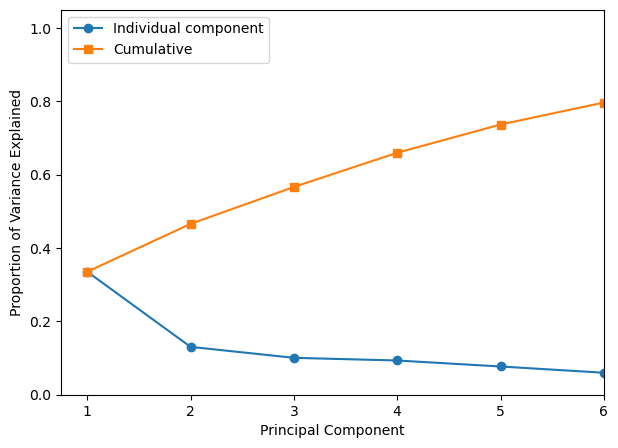
\includegraphics{assignment6111_files/figure-pdf/cell-35-output-1.png}

\begin{Shaded}
\begin{Highlighting}[]
\CommentTok{\#\#choose 2}

\NormalTok{PCA\_var}\OperatorTok{=}\BuiltInTok{sum}\NormalTok{(pca\_X.explained\_variance\_ratio\_[}\DecValTok{0}\NormalTok{:}\DecValTok{2}\NormalTok{])}
\NormalTok{PCA\_var}
\end{Highlighting}
\end{Shaded}

\begin{verbatim}
0.4659712729918205
\end{verbatim}

\begin{Shaded}
\begin{Highlighting}[]
\NormalTok{plt.figure(figsize}\OperatorTok{=}\NormalTok{(}\DecValTok{8}\NormalTok{, }\DecValTok{6}\NormalTok{))}

\NormalTok{principal\_components }\OperatorTok{=}\NormalTok{ pca\_X.fit\_transform(X)}
\NormalTok{kmeans }\OperatorTok{=}\NormalTok{ KMeans(n\_clusters}\OperatorTok{=}\DecValTok{2}\NormalTok{, n\_init}\OperatorTok{=}\DecValTok{20}\NormalTok{, random\_state}\OperatorTok{=}\DecValTok{0}\NormalTok{)}
\NormalTok{kmeans.fit(principal\_components)}
\NormalTok{cluster\_labels }\OperatorTok{=}\NormalTok{ kmeans.labels\_}

\CommentTok{\# Plot data points}
\NormalTok{plt.scatter(principal\_components[:, }\DecValTok{0}\NormalTok{], principal\_components[:, }\DecValTok{1}\NormalTok{], c}\OperatorTok{=}\NormalTok{cluster\_labels, cmap}\OperatorTok{=}\StringTok{\textquotesingle{}viridis\textquotesingle{}}\NormalTok{, edgecolors}\OperatorTok{=}\StringTok{\textquotesingle{}k\textquotesingle{}}\NormalTok{)}

\CommentTok{\# Plot cluster centers}
\NormalTok{plt.scatter(kmeans.cluster\_centers\_[:, }\DecValTok{0}\NormalTok{], kmeans.cluster\_centers\_[:, }\DecValTok{1}\NormalTok{], marker}\OperatorTok{=}\StringTok{\textquotesingle{}x\textquotesingle{}}\NormalTok{, c}\OperatorTok{=}\StringTok{\textquotesingle{}red\textquotesingle{}}\NormalTok{, s}\OperatorTok{=}\DecValTok{100}\NormalTok{, label}\OperatorTok{=}\StringTok{\textquotesingle{}Cluster Centers\textquotesingle{}}\NormalTok{)}

\NormalTok{plt.title(}\StringTok{\textquotesingle{}K{-}means Clustering Visualization (k=2)\textquotesingle{}}\NormalTok{)}
\NormalTok{plt.xlabel(}\StringTok{\textquotesingle{}Principal Component 1\textquotesingle{}}\NormalTok{)}
\NormalTok{plt.ylabel(}\StringTok{\textquotesingle{}Principal Component 2\textquotesingle{}}\NormalTok{)}
\NormalTok{plt.legend()}
\NormalTok{plt.grid(}\VariableTok{True}\NormalTok{)}
\NormalTok{plt.show()}
\end{Highlighting}
\end{Shaded}

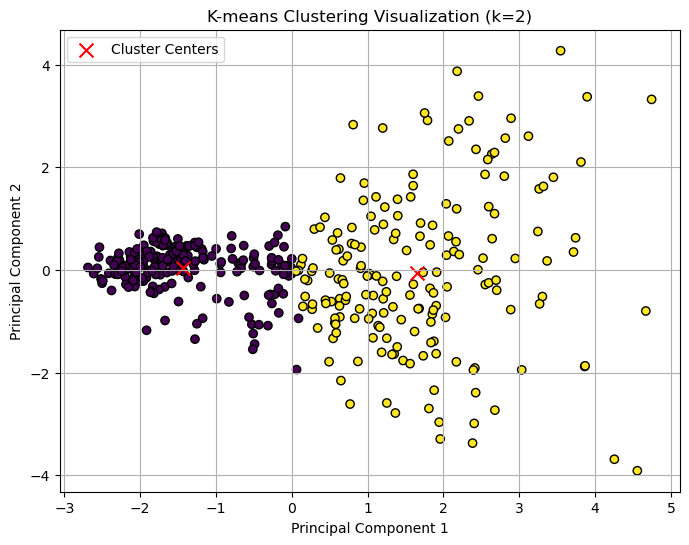
\includegraphics{assignment6111_files/figure-pdf/cell-37-output-1.png}

\begin{Shaded}
\begin{Highlighting}[]
\NormalTok{y\_1d }\OperatorTok{=}\NormalTok{ np.ravel(y\_new)}

\NormalTok{adjusted\_Rand\_index }\OperatorTok{=}\NormalTok{ adjusted\_rand\_score(y\_1d, cluster\_labels)}

\NormalTok{adjusted\_Rand\_index}
\end{Highlighting}
\end{Shaded}

\begin{verbatim}
0.4703772721070761
\end{verbatim}

\begin{itemize}
\tightlist
\item
  We choose to ue k=2, i.e.~two sub-groups, because it has a better
  average silhouette score.
\end{itemize}

\begin{enumerate}
\def\labelenumi{\arabic{enumi}.}
\setcounter{enumi}{7}
\tightlist
\item
  Data Splitting:
\end{enumerate}

\begin{Shaded}
\begin{Highlighting}[]
\NormalTok{X\_train, X\_test, y\_train, y\_test }\OperatorTok{=}\NormalTok{ train\_test\_split(}
\NormalTok{    X\_new\_dummy\_dropped, y\_new, test\_size}\OperatorTok{=}\FloatTok{0.30}\NormalTok{, random\_state}\OperatorTok{=}\DecValTok{0}\NormalTok{, stratify}\OperatorTok{=}\NormalTok{y\_new)}
\end{Highlighting}
\end{Shaded}

\begin{enumerate}
\def\labelenumi{\arabic{enumi}.}
\setcounter{enumi}{8}
\tightlist
\item
  The classifier used here is logistic regression since the predictor we
  have is catogorical with only 0 and 1 occurs, It's a natural choice
  for such tasks because it models the probability that a given input
  belongs to a particular class.
\end{enumerate}

\begin{Shaded}
\begin{Highlighting}[]
\ImportTok{import}\NormalTok{ pandas }\ImportTok{as}\NormalTok{ pd}
\ImportTok{import}\NormalTok{ numpy }\ImportTok{as}\NormalTok{ np}
\ImportTok{import}\NormalTok{ matplotlib.pyplot }\ImportTok{as}\NormalTok{ plt}
\ImportTok{import}\NormalTok{ seaborn }\ImportTok{as}\NormalTok{ sns}

\ImportTok{from}\NormalTok{ sklearn.model\_selection }\ImportTok{import}\NormalTok{ train\_test\_split, cross\_val\_score}
\ImportTok{from}\NormalTok{ sklearn.metrics }\ImportTok{import}\NormalTok{ mean\_squared\_error, confusion\_matrix, classification\_report}
\end{Highlighting}
\end{Shaded}

\begin{Shaded}
\begin{Highlighting}[]
\ImportTok{import}\NormalTok{ numpy }\ImportTok{as}\NormalTok{ np}
\ImportTok{import}\NormalTok{ pandas }\ImportTok{as}\NormalTok{ pd }
\ImportTok{import}\NormalTok{ matplotlib.pyplot }\ImportTok{as}\NormalTok{ plt}
\ImportTok{import}\NormalTok{ seaborn }\ImportTok{as}\NormalTok{ sns}
\ImportTok{from}\NormalTok{ patsy }\ImportTok{import}\NormalTok{ dmatrices, dmatrix}
\ImportTok{from}\NormalTok{ sklearn.preprocessing }\ImportTok{import}\NormalTok{ StandardScaler}
\ImportTok{from}\NormalTok{ sklearn.model\_selection }\ImportTok{import}\NormalTok{ train\_test\_split}
\ImportTok{from}\NormalTok{ sklearn }\ImportTok{import}\NormalTok{ metrics}
\ImportTok{from}\NormalTok{ sklearn.linear\_model }\ImportTok{import}\NormalTok{ LogisticRegression}
\ImportTok{from}\NormalTok{ sklearn.linear\_model }\ImportTok{import}\NormalTok{ LinearRegression}
\ImportTok{from}\NormalTok{ sklearn.metrics }\ImportTok{import}\NormalTok{ confusion\_matrix, classification\_report}
\ImportTok{import}\NormalTok{ statsmodels.api }\ImportTok{as}\NormalTok{ sm}
\ImportTok{from}\NormalTok{ sklearn.model\_selection }\ImportTok{import}\NormalTok{ train\_test\_split}
\ImportTok{from}\NormalTok{ sklearn.metrics }\ImportTok{import}\NormalTok{ confusion\_matrix, classification\_report, roc\_curve, roc\_auc\_score, accuracy\_score}
\ImportTok{from}\NormalTok{ sklearn.preprocessing }\ImportTok{import}\NormalTok{ StandardScaler}
\ImportTok{from}\NormalTok{ sklearn.tree }\ImportTok{import}\NormalTok{ DecisionTreeClassifier, DecisionTreeRegressor, plot\_tree}
\ImportTok{import}\NormalTok{ statsmodels.api }\ImportTok{as}\NormalTok{ sm}
\end{Highlighting}
\end{Shaded}

\begin{Shaded}
\begin{Highlighting}[]
\NormalTok{logistic}\OperatorTok{=}\NormalTok{ LogisticRegression(max\_iter}\OperatorTok{=}\DecValTok{2000}\NormalTok{)}
\end{Highlighting}
\end{Shaded}

\begin{Shaded}
\begin{Highlighting}[]
\NormalTok{logistic.fit(X\_train, y\_train)}
\end{Highlighting}
\end{Shaded}

\begin{verbatim}
/Users/apple/anaconda3/lib/python3.11/site-packages/sklearn/utils/validation.py:1184: DataConversionWarning: A column-vector y was passed when a 1d array was expected. Please change the shape of y to (n_samples, ), for example using ravel().
  y = column_or_1d(y, warn=True)
\end{verbatim}

\begin{verbatim}
LogisticRegression(max_iter=2000)
\end{verbatim}

\begin{Shaded}
\begin{Highlighting}[]
\NormalTok{pred\_prob }\OperatorTok{=}\NormalTok{ logistic.predict\_proba(X\_test)}
\NormalTok{pred\_prob}
\end{Highlighting}
\end{Shaded}

\begin{verbatim}
array([[1.99946545e-02, 9.80005345e-01],
       [9.99855793e-01, 1.44206948e-04],
       [9.96270637e-01, 3.72936262e-03],
       [9.95050690e-01, 4.94931023e-03],
       [9.92267311e-01, 7.73268922e-03],
       [8.76974595e-03, 9.91230254e-01],
       [9.99994874e-01, 5.12587848e-06],
       [9.99513945e-01, 4.86055442e-04],
       [9.94348624e-01, 5.65137555e-03],
       [9.98770065e-01, 1.22993511e-03],
       [9.80737022e-01, 1.92629783e-02],
       [9.94333991e-01, 5.66600943e-03],
       [4.12144797e-01, 5.87855203e-01],
       [2.28415022e-01, 7.71584978e-01],
       [2.01837620e-02, 9.79816238e-01],
       [9.99570245e-01, 4.29754516e-04],
       [1.37429750e-02, 9.86257025e-01],
       [9.99646164e-01, 3.53836413e-04],
       [8.21520533e-03, 9.91784795e-01],
       [9.99043846e-01, 9.56153647e-04],
       [9.97467722e-01, 2.53227808e-03],
       [9.94701371e-01, 5.29862926e-03],
       [8.43763661e-01, 1.56236339e-01],
       [2.31906788e-02, 9.76809321e-01],
       [9.99997272e-01, 2.72757153e-06],
       [9.99948710e-01, 5.12899659e-05],
       [4.78052762e-02, 9.52194724e-01],
       [5.85783173e-02, 9.41421683e-01],
       [2.61010438e-02, 9.73898956e-01],
       [9.99924872e-01, 7.51281208e-05],
       [9.96825804e-01, 3.17419626e-03],
       [1.98984679e-02, 9.80101532e-01],
       [9.85309958e-01, 1.46900423e-02],
       [6.23320588e-03, 9.93766794e-01],
       [9.94852349e-01, 5.14765059e-03],
       [9.98540642e-01, 1.45935844e-03],
       [5.68873193e-02, 9.43112681e-01],
       [1.20777961e-02, 9.87922204e-01],
       [9.99426883e-01, 5.73117185e-04],
       [9.99246421e-01, 7.53578680e-04],
       [9.99942229e-01, 5.77711385e-05],
       [5.89684386e-03, 9.94103156e-01],
       [9.63118764e-01, 3.68812362e-02],
       [4.85739795e-02, 9.51426020e-01],
       [7.61609113e-01, 2.38390887e-01],
       [8.19897267e-01, 1.80102733e-01],
       [1.69186805e-02, 9.83081319e-01],
       [9.72156562e-01, 2.78434382e-02],
       [9.99763052e-01, 2.36947785e-04],
       [6.05997588e-02, 9.39400241e-01],
       [8.31678165e-01, 1.68321835e-01],
       [9.97413410e-01, 2.58658988e-03],
       [7.03579443e-01, 2.96420557e-01],
       [1.55691540e-02, 9.84430846e-01],
       [9.96366834e-01, 3.63316649e-03],
       [9.99731869e-01, 2.68130700e-04],
       [9.99999498e-01, 5.02455594e-07],
       [9.99642213e-01, 3.57787289e-04],
       [2.61794596e-02, 9.73820540e-01],
       [7.68028402e-02, 9.23197160e-01],
       [9.98819507e-01, 1.18049264e-03],
       [9.99902311e-01, 9.76887922e-05],
       [9.99082960e-01, 9.17039820e-04],
       [2.37311312e-02, 9.76268869e-01],
       [9.84747176e-01, 1.52528243e-02],
       [2.25014940e-02, 9.77498506e-01],
       [9.99998716e-01, 1.28418834e-06],
       [9.61262819e-03, 9.90387372e-01],
       [5.44722125e-03, 9.94552779e-01],
       [1.67260083e-02, 9.83273992e-01],
       [9.99987762e-01, 1.22375679e-05],
       [1.49163539e-02, 9.85083646e-01],
       [2.47961761e-02, 9.75203824e-01],
       [9.98817372e-01, 1.18262807e-03],
       [9.70223647e-01, 2.97763525e-02],
       [9.99999096e-01, 9.04422666e-07],
       [9.99991601e-01, 8.39858306e-06],
       [9.89547141e-01, 1.04528590e-02],
       [2.85853969e-02, 9.71414603e-01],
       [8.77814748e-03, 9.91221853e-01],
       [5.15817716e-01, 4.84182284e-01],
       [9.99993695e-01, 6.30481387e-06],
       [9.80820426e-01, 1.91795740e-02],
       [9.99903765e-01, 9.62350519e-05],
       [9.99924807e-01, 7.51930040e-05],
       [1.16071189e-02, 9.88392881e-01],
       [2.95945919e-02, 9.70405408e-01],
       [5.04325056e-01, 4.95674944e-01],
       [1.23565046e-02, 9.87643495e-01],
       [9.99890321e-01, 1.09679206e-04],
       [9.97954098e-01, 2.04590226e-03],
       [9.99819559e-01, 1.80440857e-04],
       [9.29102878e-01, 7.08971217e-02],
       [9.83814563e-01, 1.61854366e-02],
       [9.16333637e-01, 8.36663635e-02],
       [4.91439895e-02, 9.50856011e-01],
       [1.86105635e-02, 9.81389437e-01],
       [9.99566848e-01, 4.33151516e-04],
       [1.56620894e-02, 9.84337911e-01],
       [9.99759927e-01, 2.40073306e-04],
       [9.99997724e-01, 2.27583127e-06],
       [9.99999989e-01, 1.06106622e-08],
       [9.99992224e-01, 7.77615534e-06],
       [9.22060802e-01, 7.79391984e-02],
       [1.45392287e-02, 9.85460771e-01],
       [1.92961645e-02, 9.80703835e-01],
       [9.92023173e-01, 7.97682669e-03],
       [9.98831699e-01, 1.16830117e-03],
       [1.44133996e-02, 9.85586600e-01],
       [9.82167114e-01, 1.78328857e-02],
       [7.52750281e-02, 9.24724972e-01],
       [6.76615681e-03, 9.93233843e-01],
       [5.17228552e-01, 4.82771448e-01],
       [1.28111803e-02, 9.87188820e-01],
       [5.78770899e-02, 9.42122910e-01],
       [7.31391406e-01, 2.68608594e-01],
       [9.96221371e-01, 3.77862870e-03],
       [1.10767301e-02, 9.88923270e-01],
       [9.98893379e-01, 1.10662146e-03]])
\end{verbatim}

\begin{Shaded}
\begin{Highlighting}[]
\NormalTok{y\_logist}\OperatorTok{=}\NormalTok{np.ravel(y\_test)}
\NormalTok{df }\OperatorTok{=}\NormalTok{ pd.DataFrame(data }\OperatorTok{=}\NormalTok{ \{}\StringTok{\textquotesingle{}prob\textquotesingle{}}\NormalTok{: pred\_prob[:,}\DecValTok{1}\NormalTok{], }\StringTok{\textquotesingle{}y\_test\textquotesingle{}}\NormalTok{: y\_logist\})}
\end{Highlighting}
\end{Shaded}

\begin{enumerate}
\def\labelenumi{\arabic{enumi}.}
\setcounter{enumi}{9}
\tightlist
\item
  Performance Metrics
\end{enumerate}

\begin{Shaded}
\begin{Highlighting}[]
\NormalTok{df[}\StringTok{\textquotesingle{}y\_test\_pred\textquotesingle{}}\NormalTok{] }\OperatorTok{=}\NormalTok{ df.prob.}\BuiltInTok{map}\NormalTok{(}\KeywordTok{lambda}\NormalTok{ x: }\DecValTok{1} \ControlFlowTok{if}\NormalTok{ x}\OperatorTok{\textgreater{}}\FloatTok{0.5} \ControlFlowTok{else} \DecValTok{0}\NormalTok{)}
\end{Highlighting}
\end{Shaded}

\begin{Shaded}
\begin{Highlighting}[]
\NormalTok{cm }\OperatorTok{=}\NormalTok{ confusion\_matrix(df.y\_test, df.y\_test\_pred)}
\BuiltInTok{print}\NormalTok{(}\StringTok{\textquotesingle{}Confusion Matrix : }\CharTok{\textbackslash{}n}\StringTok{\textquotesingle{}}\NormalTok{, cm)}
\NormalTok{total }\OperatorTok{=} \BuiltInTok{sum}\NormalTok{(}\BuiltInTok{sum}\NormalTok{(cm))}
\NormalTok{accuracy }\OperatorTok{=}\NormalTok{ (cm[}\DecValTok{0}\NormalTok{,}\DecValTok{0}\NormalTok{]}\OperatorTok{+}\NormalTok{cm[}\DecValTok{1}\NormalTok{,}\DecValTok{1}\NormalTok{])}\OperatorTok{/}\NormalTok{total}
\BuiltInTok{print}\NormalTok{ (}\StringTok{\textquotesingle{}Accuracy : \textquotesingle{}}\NormalTok{, accuracy)}
\end{Highlighting}
\end{Shaded}

\begin{verbatim}
Confusion Matrix : 
 [[72  2]
 [ 2 43]]
Accuracy :  0.9663865546218487
\end{verbatim}

\begin{Shaded}
\begin{Highlighting}[]
\NormalTok{sensitivity }\OperatorTok{=}\NormalTok{ cm[}\DecValTok{1}\NormalTok{,}\DecValTok{1}\NormalTok{]}\OperatorTok{/}\NormalTok{(cm[}\DecValTok{1}\NormalTok{,}\DecValTok{0}\NormalTok{]}\OperatorTok{+}\NormalTok{cm[}\DecValTok{1}\NormalTok{,}\DecValTok{1}\NormalTok{])}
\BuiltInTok{print}\NormalTok{(}\StringTok{\textquotesingle{}Sensitivity : \textquotesingle{}}\NormalTok{, sensitivity )}
\NormalTok{specificity }\OperatorTok{=}\NormalTok{ cm[}\DecValTok{0}\NormalTok{,}\DecValTok{0}\NormalTok{]}\OperatorTok{/}\NormalTok{(cm[}\DecValTok{0}\NormalTok{,}\DecValTok{0}\NormalTok{]}\OperatorTok{+}\NormalTok{cm[}\DecValTok{0}\NormalTok{,}\DecValTok{1}\NormalTok{])}
\BuiltInTok{print}\NormalTok{(}\StringTok{\textquotesingle{}Specificity : \textquotesingle{}}\NormalTok{, specificity)}
\end{Highlighting}
\end{Shaded}

\begin{verbatim}
Sensitivity :  0.9555555555555556
Specificity :  0.972972972972973
\end{verbatim}

we use the sensitivity and specificity to examine the performance of the
model, sensitivity states of all the actual positive cases, how many did
the model correctly identify, and specifity states Of all the actual
negative cases, how many did the model correctly identify.

In this case, we have both of these value is relatively high, so the
model predict 1 well, which is s good model to choose.

\begin{enumerate}
\def\labelenumi{\arabic{enumi}.}
\setcounter{enumi}{10}
\tightlist
\item
  feature selection using chaning threshhold, find the best threshold.
\end{enumerate}

\begin{Shaded}
\begin{Highlighting}[]
\ImportTok{from}\NormalTok{ sklearn.linear\_model }\ImportTok{import}\NormalTok{ LassoCV}
\ImportTok{from}\NormalTok{ sklearn.feature\_selection }\ImportTok{import}\NormalTok{ SelectFromModel}



\CommentTok{\# Select features based on non{-}zero coefficients from Lasso model}
\NormalTok{feature\_selector }\OperatorTok{=}\NormalTok{ SelectFromModel(logistic, prefit}\OperatorTok{=}\VariableTok{True}\NormalTok{)}
\NormalTok{X\_train\_selected }\OperatorTok{=}\NormalTok{ feature\_selector.transform(X\_train)}
\NormalTok{X\_test\_selected }\OperatorTok{=}\NormalTok{ feature\_selector.transform(X\_test)}

\CommentTok{\# Get selected feature indices}
\NormalTok{selected\_feature\_indices }\OperatorTok{=}\NormalTok{ feature\_selector.get\_support(indices}\OperatorTok{=}\VariableTok{True}\NormalTok{)}

\CommentTok{\# Print selected feature indices}
\BuiltInTok{print}\NormalTok{(}\StringTok{"Selected feature indices:"}\NormalTok{, selected\_feature\_indices)}
\end{Highlighting}
\end{Shaded}

\begin{verbatim}
Selected feature indices: [ 2  3  5  9 12 13 16]
\end{verbatim}

\begin{verbatim}
/Users/apple/anaconda3/lib/python3.11/site-packages/sklearn/base.py:457: UserWarning: X has feature names, but SelectFromModel was fitted without feature names
  warnings.warn(
/Users/apple/anaconda3/lib/python3.11/site-packages/sklearn/base.py:457: UserWarning: X has feature names, but SelectFromModel was fitted without feature names
  warnings.warn(
\end{verbatim}

\begin{Shaded}
\begin{Highlighting}[]
\NormalTok{selected\_feature\_indices}\OperatorTok{=}\NormalTok{[}\DecValTok{2}\NormalTok{, }\DecValTok{3}\NormalTok{, }\DecValTok{5}\NormalTok{, }\DecValTok{9}\NormalTok{, }\DecValTok{12}\NormalTok{, }\DecValTok{13}\NormalTok{, }\DecValTok{16}\NormalTok{]}
\NormalTok{selected\_feature\_names }\OperatorTok{=}\NormalTok{ X\_train.columns[selected\_feature\_indices]}
\BuiltInTok{print}\NormalTok{(}\StringTok{"Selected feature names:"}\NormalTok{, selected\_feature\_names)}
\end{Highlighting}
\end{Shaded}

\begin{verbatim}
Selected feature names: Index(['sg', 'al', 'rbc', 'bgr', 'htn', 'dm', 'pe'], dtype='object')
\end{verbatim}

\begin{Shaded}
\begin{Highlighting}[]
\NormalTok{fpr, tpr, thresholds }\OperatorTok{=}\NormalTok{ roc\_curve(df.y\_test, df.prob)}
\NormalTok{ks\_statistic }\OperatorTok{=}\NormalTok{ np.}\BuiltInTok{max}\NormalTok{(tpr }\OperatorTok{{-}}\NormalTok{ fpr)}
\NormalTok{ks\_threshold }\OperatorTok{=}\NormalTok{ thresholds[np.argmax(tpr }\OperatorTok{{-}}\NormalTok{ fpr)]}
\NormalTok{ks\_threshold}
\end{Highlighting}
\end{Shaded}

\begin{verbatim}
0.482771448068781
\end{verbatim}

\begin{Shaded}
\begin{Highlighting}[]
\NormalTok{df[}\StringTok{\textquotesingle{}y\_test\_pred2\textquotesingle{}}\NormalTok{] }\OperatorTok{=}\NormalTok{ df.prob.}\BuiltInTok{map}\NormalTok{(}\KeywordTok{lambda}\NormalTok{ x: }\DecValTok{1} \ControlFlowTok{if}\NormalTok{ x}\OperatorTok{\textgreater{}}\NormalTok{ks\_threshold }\ControlFlowTok{else} \DecValTok{0}\NormalTok{)}
\NormalTok{cm1 }\OperatorTok{=}\NormalTok{ confusion\_matrix(df.y\_test, df.y\_test\_pred2)}
\NormalTok{sensitivity\_log }\OperatorTok{=}\NormalTok{ cm1[}\DecValTok{1}\NormalTok{,}\DecValTok{1}\NormalTok{]}\OperatorTok{/}\NormalTok{(cm1[}\DecValTok{1}\NormalTok{,}\DecValTok{0}\NormalTok{]}\OperatorTok{+}\NormalTok{cm1[}\DecValTok{1}\NormalTok{,}\DecValTok{1}\NormalTok{])}
\BuiltInTok{print}\NormalTok{(}\StringTok{\textquotesingle{}Sensitivity : \textquotesingle{}}\NormalTok{, sensitivity\_log )}
\NormalTok{specificity\_log }\OperatorTok{=}\NormalTok{ cm1[}\DecValTok{0}\NormalTok{,}\DecValTok{0}\NormalTok{]}\OperatorTok{/}\NormalTok{(cm1[}\DecValTok{0}\NormalTok{,}\DecValTok{0}\NormalTok{]}\OperatorTok{+}\NormalTok{cm1[}\DecValTok{0}\NormalTok{,}\DecValTok{1}\NormalTok{])}
\BuiltInTok{print}\NormalTok{(}\StringTok{\textquotesingle{}Specificity : \textquotesingle{}}\NormalTok{, specificity\_log)}
\NormalTok{acc\_log }\OperatorTok{=}\NormalTok{ accuracy\_score(df.y\_test, df.y\_test\_pred2)}
\NormalTok{acc\_log}
\end{Highlighting}
\end{Shaded}

\begin{verbatim}
Sensitivity :  0.9777777777777777
Specificity :  0.9594594594594594
\end{verbatim}

\begin{verbatim}
0.9663865546218487
\end{verbatim}

hence the accuracy has incease, since sensitivity increase little, which
correctly identify more 1.

\begin{Shaded}
\begin{Highlighting}[]
\NormalTok{logistic.coef\_}
\end{Highlighting}
\end{Shaded}

\begin{verbatim}
array([[ 0.15134758, -0.72220478,  1.39266695, -2.1794434 , -0.17536635,
         1.90791624, -0.49063808, -0.28623345, -0.24913584, -1.0606856 ,
        -0.34233395, -0.72952786, -1.06557624, -0.98789526, -0.04331981,
         0.75457121, -1.05807497, -0.72070879]])
\end{verbatim}

\begin{Shaded}
\begin{Highlighting}[]
\NormalTok{X\_new\_1 }\OperatorTok{=}\NormalTok{ dmatrix(}
\StringTok{\textquotesingle{}sg + al + rbc +bgr+htn+dm+pe\textquotesingle{}}\NormalTok{,}
\NormalTok{data}\OperatorTok{=}\NormalTok{X\_new\_dummy\_dropped,}
\NormalTok{return\_type}\OperatorTok{=}\StringTok{\textquotesingle{}dataframe\textquotesingle{}}
\NormalTok{)}

\NormalTok{X\_new\_1}
\end{Highlighting}
\end{Shaded}

\begin{longtable}[]{@{}lllllllll@{}}
\toprule\noalign{}
& Intercept & sg & al & rbc & bgr & htn & dm & pe \\
\midrule\noalign{}
\endhead
\bottomrule\noalign{}
\endlastfoot
0 & 1.0 & 0.454071 & -0.012548 & -1.0 & -0.341498 & 1.0 & 1.0 & 0.0 \\
1 & 1.0 & 0.454071 & 2.208413 & -1.0 & -0.740638 & 0.0 & 0.0 & 0.0 \\
2 & 1.0 & -1.297699 & 0.727772 & 1.0 & 3.473064 & 0.0 & 1.0 & 0.0 \\
3 & 1.0 & -2.173584 & 2.208413 & 1.0 & -0.392022 & 1.0 & 0.0 & 1.0 \\
4 & 1.0 & -1.297699 & 0.727772 & 1.0 & -0.530963 & 0.0 & 0.0 & 0.0 \\
... & ... & ... & ... & ... & ... & ... & ... & ... \\
395 & 1.0 & 0.454071 & -0.752868 & 1.0 & -0.101509 & 0.0 & 0.0 & 0.0 \\
396 & 1.0 & 1.329955 & -0.752868 & 1.0 & -0.922524 & 0.0 & 0.0 & 0.0 \\
397 & 1.0 & 0.454071 & -0.752868 & 1.0 & -0.606749 & 0.0 & 0.0 & 0.0 \\
398 & 1.0 & 1.329955 & -0.752868 & 1.0 & -0.429915 & 0.0 & 0.0 & 0.0 \\
399 & 1.0 & 1.329955 & -0.752868 & 1.0 & -0.215188 & 0.0 & 0.0 & 0.0 \\
\end{longtable}

\begin{Shaded}
\begin{Highlighting}[]
\NormalTok{X\_train\_new, X\_test\_new, y\_train\_new, y\_test\_new }\OperatorTok{=}\NormalTok{ train\_test\_split(}
\NormalTok{    X\_new\_1, y\_new, train\_size}\OperatorTok{=}\FloatTok{0.7}\NormalTok{, random\_state}\OperatorTok{=}\DecValTok{1}\NormalTok{, stratify}\OperatorTok{=}\NormalTok{y\_new)}

\NormalTok{model }\OperatorTok{=}\NormalTok{ sm.Logit(y\_train\_new, X\_train\_new).fit()}

\NormalTok{model.summary()}
\end{Highlighting}
\end{Shaded}

\begin{verbatim}
/Users/apple/anaconda3/lib/python3.11/site-packages/statsmodels/base/model.py:607: ConvergenceWarning: Maximum Likelihood optimization failed to converge. Check mle_retvals
  warnings.warn("Maximum Likelihood optimization failed to "
\end{verbatim}

\begin{verbatim}
Warning: Maximum number of iterations has been exceeded.
         Current function value: 0.032794
         Iterations: 35
\end{verbatim}

\begin{center}
\begin{tabular}{lclc}
\toprule
\textbf{Dep. Variable:}   &      class       & \textbf{  No. Observations:  } &      277    \\
\textbf{Model:}           &      Logit       & \textbf{  Df Residuals:      } &      269    \\
\textbf{Method:}          &       MLE        & \textbf{  Df Model:          } &        7    \\
\textbf{Date:}            & Thu, 18 Apr 2024 & \textbf{  Pseudo R-squ.:     } &   0.9506    \\
\textbf{Time:}            &     21:09:11     & \textbf{  Log-Likelihood:    } &   -9.0839   \\
\textbf{converged:}       &      False       & \textbf{  LL-Null:           } &   -183.82   \\
\textbf{Covariance Type:} &    nonrobust     & \textbf{  LLR p-value:       } & 1.602e-71   \\
\bottomrule
\end{tabular}
\begin{tabular}{lcccccc}
                   & \textbf{coef} & \textbf{std err} & \textbf{z} & \textbf{P$> |$z$|$} & \textbf{[0.025} & \textbf{0.975]}  \\
\midrule
\textbf{Intercept} &      -6.9247  &        3.008     &    -2.302  &         0.021        &      -12.820    &       -1.030     \\
\textbf{sg}        &       5.5989  &        2.657     &     2.108  &         0.035        &        0.392    &       10.806     \\
\textbf{al}        &      -7.2713  &        2.377     &    -3.059  &         0.002        &      -11.930    &       -2.612     \\
\textbf{rbc}       &       1.8657  &        0.786     &     2.374  &         0.018        &        0.326    &        3.406     \\
\textbf{bgr}       &      -3.4110  &        2.595     &    -1.315  &         0.189        &       -8.497    &        1.675     \\
\textbf{htn}       &     -26.4113  &     2.09e+06     & -1.26e-05  &         1.000        &     -4.1e+06    &      4.1e+06     \\
\textbf{dm}        &    -106.3805  &     5.74e+23     & -1.85e-22  &         1.000        &    -1.12e+24    &     1.12e+24     \\
\textbf{pe}        &     -22.5895  &     2.25e+04     &    -0.001  &         0.999        &    -4.42e+04    &     4.42e+04     \\
\bottomrule
\end{tabular}
%\caption{Logit Regression Results}
\end{center}

Possibly complete quasi-separation: A fraction 0.66 of observations can be \newline
 perfectly predicted. This might indicate that there is complete \newline
 quasi-separation. In this case some parameters will not be identified.

\begin{enumerate}
\def\labelenumi{\arabic{enumi}.}
\item
  From the given chart, we see that only the ``sg'', ``al'' and ``rbc''
  has p value less then 0.05, so they are the significent variable among
  the variables we choose, the other variables are having too large p
  value, become not significent.
\item
  From thses 3 vriables, ``sg'' has the larget positve coefficent, which
  means the most factor which would increase the rate of Chronic Kidney
  Disease is specific gravity, and the more albumin will be, the less
  probabilty of having Chronic Kidney Disease.
\end{enumerate}

Dicision Tree (9\textasciitilde11):

\begin{itemize}
\tightlist
\item
  There are a few reasons why we use Decision Tree. First, we realize
  that the predicted value follows binary distribution so we use
  Classification Tree to predict the discrete label. In addition, the
  Decision Tree can be used for handling mixed data types, which match
  the situation of our dataset.
\end{itemize}

\begin{Shaded}
\begin{Highlighting}[]
\NormalTok{decision\_tree }\OperatorTok{=}\NormalTok{ DecisionTreeClassifier(}
\NormalTok{    max\_depth }\OperatorTok{=} \DecValTok{30}\NormalTok{, }
\NormalTok{    random\_state}\OperatorTok{=}\DecValTok{1}\NormalTok{)}
\end{Highlighting}
\end{Shaded}

\begin{Shaded}
\begin{Highlighting}[]
\NormalTok{decision\_tree.fit(X\_train, y\_train)}
\end{Highlighting}
\end{Shaded}

\begin{verbatim}
DecisionTreeClassifier(max_depth=30, random_state=1)
\end{verbatim}

\begin{Shaded}
\begin{Highlighting}[]
\NormalTok{fig, axes }\OperatorTok{=}\NormalTok{ plt.subplots(}
\NormalTok{    nrows }\OperatorTok{=} \DecValTok{1}\NormalTok{,ncols }\OperatorTok{=} \DecValTok{1}\NormalTok{,figsize }\OperatorTok{=}\NormalTok{ (}\DecValTok{5}\NormalTok{,}\DecValTok{5}\NormalTok{), dpi}\OperatorTok{=}\DecValTok{300}
\NormalTok{    )}
\NormalTok{plot\_tree(}
\NormalTok{    decision\_tree, }
\NormalTok{    max\_depth}\OperatorTok{=} \DecValTok{40}\NormalTok{, }
\NormalTok{    feature\_names }\OperatorTok{=}\NormalTok{ X\_train.columns.tolist(), }
\NormalTok{    class\_names}\OperatorTok{=}\NormalTok{[}\StringTok{\textquotesingle{}notckd\textquotesingle{}}\NormalTok{, }\StringTok{\textquotesingle{}ckd\textquotesingle{}}\NormalTok{],}
\NormalTok{    filled }\OperatorTok{=} \VariableTok{True}
\NormalTok{)}
\end{Highlighting}
\end{Shaded}

\begin{verbatim}
[Text(0.5714285714285714, 0.9166666666666666, 'sg <= 0.366\ngini = 0.471\nsamples = 277\nvalue = [172, 105]\nclass = notckd'),
 Text(0.42857142857142855, 0.75, 'gini = 0.0\nsamples = 148\nvalue = [148, 0]\nclass = notckd'),
 Text(0.7142857142857143, 0.75, 'al <= -0.235\ngini = 0.303\nsamples = 129\nvalue = [24, 105]\nclass = ckd'),
 Text(0.5714285714285714, 0.5833333333333334, 'sc <= -0.318\ngini = 0.102\nsamples = 111\nvalue = [6, 105]\nclass = ckd'),
 Text(0.42857142857142855, 0.4166666666666667, 'rbc <= 0.0\ngini = 0.019\nsamples = 106\nvalue = [1, 105]\nclass = ckd'),
 Text(0.2857142857142857, 0.25, 'bp <= -0.107\ngini = 0.219\nsamples = 8\nvalue = [1, 7]\nclass = ckd'),
 Text(0.14285714285714285, 0.08333333333333333, 'gini = 0.0\nsamples = 7\nvalue = [0, 7]\nclass = ckd'),
 Text(0.42857142857142855, 0.08333333333333333, 'gini = 0.0\nsamples = 1\nvalue = [1, 0]\nclass = notckd'),
 Text(0.5714285714285714, 0.25, 'gini = 0.0\nsamples = 98\nvalue = [0, 98]\nclass = ckd'),
 Text(0.7142857142857143, 0.4166666666666667, 'gini = 0.0\nsamples = 5\nvalue = [5, 0]\nclass = notckd'),
 Text(0.8571428571428571, 0.5833333333333334, 'gini = 0.0\nsamples = 18\nvalue = [18, 0]\nclass = notckd')]
\end{verbatim}

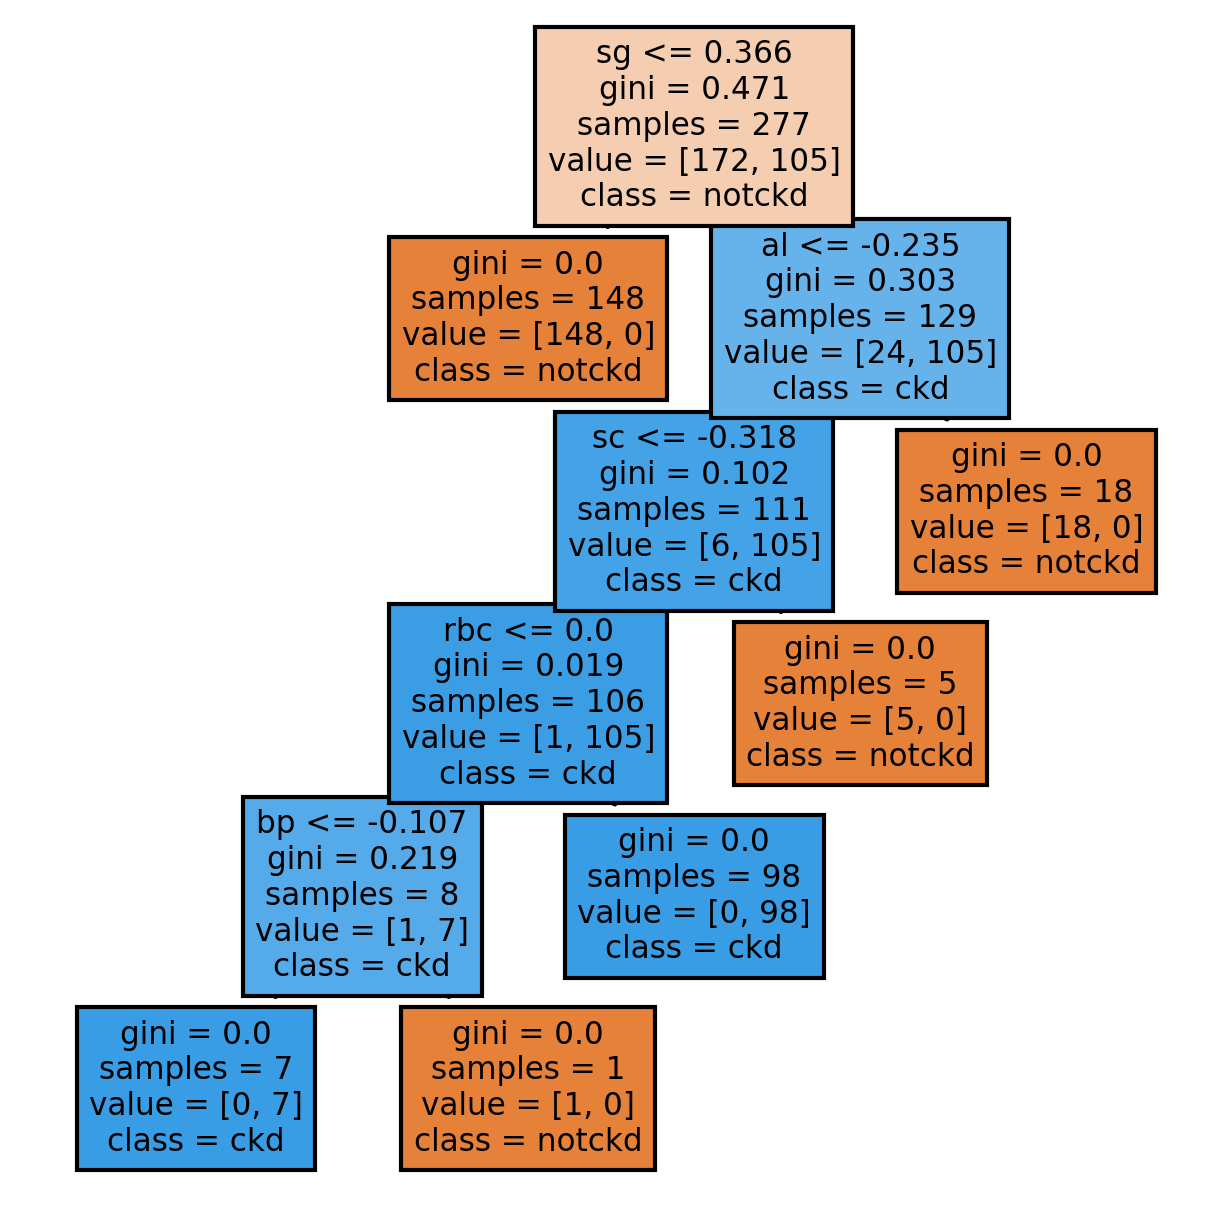
\includegraphics{assignment6111_files/figure-pdf/cell-58-output-2.png}

\begin{Shaded}
\begin{Highlighting}[]
\NormalTok{pred }\OperatorTok{=}\NormalTok{ decision\_tree.predict(X\_test)}

\NormalTok{pred[:}\DecValTok{5}\NormalTok{]}
\end{Highlighting}
\end{Shaded}

\begin{verbatim}
array([1, 0, 0, 0, 0], dtype=int8)
\end{verbatim}

\begin{Shaded}
\begin{Highlighting}[]
\NormalTok{con\_matrix }\OperatorTok{=}\NormalTok{ confusion\_matrix(y\_test, pred)}
\NormalTok{cm }\OperatorTok{=}\NormalTok{ pd.DataFrame(con\_matrix, index}\OperatorTok{=}\NormalTok{[}\StringTok{\textquotesingle{}notckd\textquotesingle{}}\NormalTok{, }\StringTok{\textquotesingle{}ckd\textquotesingle{}}\NormalTok{], columns}\OperatorTok{=}\NormalTok{[}\StringTok{\textquotesingle{}notckd\textquotesingle{}}\NormalTok{, }\StringTok{\textquotesingle{}ckd\textquotesingle{}}\NormalTok{])}
\NormalTok{cm.index.name }\OperatorTok{=} \StringTok{\textquotesingle{}True\textquotesingle{}}
\NormalTok{cm.columns.name }\OperatorTok{=} \StringTok{\textquotesingle{}Predicted\textquotesingle{}}
\NormalTok{cm}
\end{Highlighting}
\end{Shaded}

\begin{longtable}[]{@{}lll@{}}
\toprule\noalign{}
Predicted & notckd & ckd \\
True & & \\
\midrule\noalign{}
\endhead
\bottomrule\noalign{}
\endlastfoot
notckd & 73 & 1 \\
ckd & 2 & 43 \\
\end{longtable}

\begin{Shaded}
\begin{Highlighting}[]
\NormalTok{sensitivity }\OperatorTok{=}\NormalTok{ con\_matrix[}\DecValTok{1}\NormalTok{,}\DecValTok{1}\NormalTok{]}\OperatorTok{/}\NormalTok{(con\_matrix[}\DecValTok{1}\NormalTok{,}\DecValTok{0}\NormalTok{]}\OperatorTok{+}\NormalTok{con\_matrix[}\DecValTok{1}\NormalTok{,}\DecValTok{1}\NormalTok{])}
\BuiltInTok{print}\NormalTok{(}\StringTok{\textquotesingle{}Sensitivity : \textquotesingle{}}\NormalTok{, sensitivity)}

\NormalTok{specificity }\OperatorTok{=}\NormalTok{ con\_matrix[}\DecValTok{0}\NormalTok{,}\DecValTok{0}\NormalTok{]}\OperatorTok{/}\NormalTok{(con\_matrix[}\DecValTok{0}\NormalTok{,}\DecValTok{0}\NormalTok{]}\OperatorTok{+}\NormalTok{con\_matrix[}\DecValTok{0}\NormalTok{,}\DecValTok{1}\NormalTok{])}
\BuiltInTok{print}\NormalTok{(}\StringTok{\textquotesingle{}Specificity : \textquotesingle{}}\NormalTok{, specificity )}
\end{Highlighting}
\end{Shaded}

\begin{verbatim}
Sensitivity :  0.9555555555555556
Specificity :  0.9864864864864865
\end{verbatim}

\begin{Shaded}
\begin{Highlighting}[]
\NormalTok{decision\_tree.score(X\_test, y\_test)}
\end{Highlighting}
\end{Shaded}

\begin{verbatim}
0.9747899159663865
\end{verbatim}

\begin{Shaded}
\begin{Highlighting}[]
\BuiltInTok{print}\NormalTok{(classification\_report(y\_test, pred))}
\end{Highlighting}
\end{Shaded}

\begin{verbatim}
              precision    recall  f1-score   support

           0       0.97      0.99      0.98        74
           1       0.98      0.96      0.97        45

    accuracy                           0.97       119
   macro avg       0.98      0.97      0.97       119
weighted avg       0.97      0.97      0.97       119
\end{verbatim}

\begin{itemize}
\tightlist
\item
  From the output above, we can see that the precision of ckd is 0.97,
  which means 97\% of the samples predicted as ``ckd'' are actually
  ``ckd''. And the precision of ``notckd'' is 0.98, which means 98\% of
  the sampels predicted as ``notckd'' are correctly identified.
\end{itemize}

\begin{enumerate}
\def\labelenumi{\arabic{enumi}.}
\setcounter{enumi}{10}
\tightlist
\item
  To get a better performance of decision tree
\end{enumerate}

\begin{Shaded}
\begin{Highlighting}[]
\NormalTok{path }\OperatorTok{=}\NormalTok{ decision\_tree.cost\_complexity\_pruning\_path(}
\NormalTok{    X\_train, }
\NormalTok{    y\_train}
\NormalTok{)}
\NormalTok{ccp\_alphas, impurities }\OperatorTok{=}\NormalTok{ path.ccp\_alphas, path.impurities}
\end{Highlighting}
\end{Shaded}

\begin{Shaded}
\begin{Highlighting}[]
\NormalTok{clfs }\OperatorTok{=}\NormalTok{ [] }\CommentTok{\# save fitted trees with different alphas}
\ControlFlowTok{for}\NormalTok{ ccp\_alpha }\KeywordTok{in}\NormalTok{ ccp\_alphas:}
\NormalTok{    clf }\OperatorTok{=}\NormalTok{ DecisionTreeClassifier(}
\NormalTok{        random\_state}\OperatorTok{=}\DecValTok{1}\NormalTok{, }
\NormalTok{        ccp\_alpha}\OperatorTok{=}\NormalTok{ccp\_alpha}
\NormalTok{        )}
\NormalTok{    clf.fit(X\_train, y\_train)}
\NormalTok{    clfs.append(clf)}

\NormalTok{depth }\OperatorTok{=}\NormalTok{ [clf.tree\_.max\_depth }\ControlFlowTok{for}\NormalTok{ clf }\KeywordTok{in}\NormalTok{ clfs]}
\NormalTok{depth}
\end{Highlighting}
\end{Shaded}

\begin{verbatim}
[5, 3, 2, 1, 0]
\end{verbatim}

\begin{Shaded}
\begin{Highlighting}[]
\NormalTok{test\_score }\OperatorTok{=}\NormalTok{ [clf.score(X\_test, y\_test) }\ControlFlowTok{for}\NormalTok{ clf }\KeywordTok{in}\NormalTok{ clfs]}
\end{Highlighting}
\end{Shaded}

\begin{Shaded}
\begin{Highlighting}[]
\NormalTok{plt.plot(depth, test\_score)}
\NormalTok{plt.xlabel(}\StringTok{\textquotesingle{}Depth\textquotesingle{}}\NormalTok{)}
\NormalTok{plt.ylabel(}\StringTok{\textquotesingle{}Accuracy\textquotesingle{}}\NormalTok{)}
\NormalTok{plt.show()}
\end{Highlighting}
\end{Shaded}

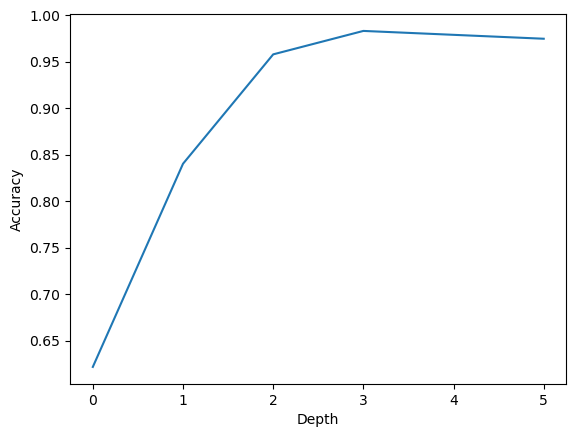
\includegraphics{assignment6111_files/figure-pdf/cell-67-output-1.png}

\begin{Shaded}
\begin{Highlighting}[]
\NormalTok{cs\_dt\_best }\OperatorTok{=}\NormalTok{ DecisionTreeClassifier(}
\NormalTok{    max\_depth }\OperatorTok{=} \DecValTok{3}\NormalTok{, }
\NormalTok{    random\_state}\OperatorTok{=}\DecValTok{1}
\NormalTok{    ) }

\NormalTok{cs\_dt\_best.fit(X\_new\_dummy\_dropped, y\_new)}
\end{Highlighting}
\end{Shaded}

\begin{verbatim}
DecisionTreeClassifier(max_depth=3, random_state=1)
\end{verbatim}

\begin{Shaded}
\begin{Highlighting}[]
\NormalTok{pred }\OperatorTok{=}\NormalTok{ cs\_dt\_best.predict(X\_test)}
\NormalTok{con\_matrix2 }\OperatorTok{=}\NormalTok{ confusion\_matrix(y\_test, pred)}
\NormalTok{cmnew }\OperatorTok{=}\NormalTok{ pd.DataFrame(con\_matrix2, index}\OperatorTok{=}\NormalTok{[}\StringTok{\textquotesingle{}0\textquotesingle{}}\NormalTok{, }\StringTok{\textquotesingle{}1\textquotesingle{}}\NormalTok{], columns}\OperatorTok{=}\NormalTok{[}\StringTok{\textquotesingle{}0\textquotesingle{}}\NormalTok{, }\StringTok{\textquotesingle{}1\textquotesingle{}}\NormalTok{])}
\NormalTok{cmnew.index.name }\OperatorTok{=} \StringTok{\textquotesingle{}True\textquotesingle{}}
\NormalTok{cmnew.columns.name }\OperatorTok{=} \StringTok{\textquotesingle{}Predicted\textquotesingle{}}
\NormalTok{cmnew}
\end{Highlighting}
\end{Shaded}

\begin{longtable}[]{@{}lll@{}}
\toprule\noalign{}
Predicted & 0 & 1 \\
True & & \\
\midrule\noalign{}
\endhead
\bottomrule\noalign{}
\endlastfoot
0 & 73 & 1 \\
1 & 0 & 45 \\
\end{longtable}

\begin{Shaded}
\begin{Highlighting}[]
\NormalTok{sensitivity\_tree }\OperatorTok{=}\NormalTok{ con\_matrix2[}\DecValTok{1}\NormalTok{,}\DecValTok{1}\NormalTok{]}\OperatorTok{/}\NormalTok{(con\_matrix2[}\DecValTok{1}\NormalTok{,}\DecValTok{0}\NormalTok{]}\OperatorTok{+}\NormalTok{con\_matrix2[}\DecValTok{1}\NormalTok{,}\DecValTok{1}\NormalTok{])}
\BuiltInTok{print}\NormalTok{(}\StringTok{\textquotesingle{}Sensitivity : \textquotesingle{}}\NormalTok{, sensitivity\_tree)}

\NormalTok{specificity\_tree }\OperatorTok{=}\NormalTok{ con\_matrix2[}\DecValTok{0}\NormalTok{,}\DecValTok{0}\NormalTok{]}\OperatorTok{/}\NormalTok{(con\_matrix2[}\DecValTok{0}\NormalTok{,}\DecValTok{0}\NormalTok{]}\OperatorTok{+}\NormalTok{con\_matrix2[}\DecValTok{0}\NormalTok{,}\DecValTok{1}\NormalTok{])}
\BuiltInTok{print}\NormalTok{(}\StringTok{\textquotesingle{}Specificity : \textquotesingle{}}\NormalTok{, specificity\_tree )}
\end{Highlighting}
\end{Shaded}

\begin{verbatim}
Sensitivity :  1.0
Specificity :  0.9864864864864865
\end{verbatim}

\begin{Shaded}
\begin{Highlighting}[]
\NormalTok{acc\_tree }\OperatorTok{=}\NormalTok{ decision\_tree.score(X\_test, y\_test)}
\NormalTok{acc\_tree}
\end{Highlighting}
\end{Shaded}

\begin{verbatim}
0.9747899159663865
\end{verbatim}

\begin{Shaded}
\begin{Highlighting}[]
\BuiltInTok{print}\NormalTok{(classification\_report(y\_test, pred))}
\end{Highlighting}
\end{Shaded}

\begin{verbatim}
              precision    recall  f1-score   support

           0       1.00      0.99      0.99        74
           1       0.98      1.00      0.99        45

    accuracy                           0.99       119
   macro avg       0.99      0.99      0.99       119
weighted avg       0.99      0.99      0.99       119
\end{verbatim}

\begin{itemize}
\tightlist
\item
  We use Pruning Tree to and the number of nods for each \(\alpha\), and
  use accuracy to prue the tree. After that we test accuracy is maximum
  at depth 3 and fit it again. We can see there is an improvement on the
  precision, and Specificity\&Sensitivity .
\end{itemize}

\begin{enumerate}
\def\labelenumi{\arabic{enumi}.}
\setcounter{enumi}{11}
\tightlist
\item
  Classifier Comparison:
\end{enumerate}

\begin{Shaded}
\begin{Highlighting}[]
\NormalTok{data }\OperatorTok{=}\NormalTok{ \{}
    \StringTok{\textquotesingle{}specificity\textquotesingle{}}\NormalTok{: [specificity\_log, specificity\_tree],}
    \StringTok{\textquotesingle{}sensitivity\textquotesingle{}}\NormalTok{: [sensitivity\_log, sensitivity\_tree],}
    \StringTok{\textquotesingle{}accuracy\textquotesingle{}}\NormalTok{: [acc\_log, acc\_tree]}
\NormalTok{\}}
\NormalTok{sen\_spe }\OperatorTok{=}\NormalTok{ pd.DataFrame(data, index}\OperatorTok{=}\NormalTok{[}\StringTok{\textquotesingle{}logistic\_reg\textquotesingle{}}\NormalTok{, }\StringTok{\textquotesingle{}decision\_tree\textquotesingle{}}\NormalTok{])}
\NormalTok{sen\_spe}
\end{Highlighting}
\end{Shaded}

\begin{longtable}[]{@{}llll@{}}
\toprule\noalign{}
& specificity & sensitivity & accuracy \\
\midrule\noalign{}
\endhead
\bottomrule\noalign{}
\endlastfoot
logistic\_reg & 0.959459 & 0.977778 & 0.966387 \\
decision\_tree & 0.986486 & 1.000000 & 0.974790 \\
\end{longtable}

\begin{itemize}
\tightlist
\item
  Comparaing the Specificity\&Sensitivity and accuracy for two
  classifiers. We can see obviously that the Decision Tre has a better
  performance, so we choose the Decision Tree as our final model.
\end{itemize}

\begin{enumerate}
\def\labelenumi{\arabic{enumi}.}
\setcounter{enumi}{12}
\tightlist
\item
  Interpretable Classifier Insight: feature importance
\end{enumerate}

\begin{Shaded}
\begin{Highlighting}[]
\NormalTok{fea\_imp }\OperatorTok{=}\NormalTok{ cs\_dt\_best.feature\_importances\_}

\NormalTok{sorted\_indices }\OperatorTok{=}\NormalTok{ fea\_imp.argsort()[::}\OperatorTok{{-}}\DecValTok{1}\NormalTok{]}
\NormalTok{sorted\_feature\_names }\OperatorTok{=}\NormalTok{ X\_train.columns[sorted\_indices]}
\NormalTok{sorted\_importances }\OperatorTok{=}\NormalTok{ fea\_imp[sorted\_indices]}

\NormalTok{sns.barplot(x }\OperatorTok{=}\NormalTok{ sorted\_importances, y }\OperatorTok{=}\NormalTok{ sorted\_feature\_names)}
\NormalTok{plt.show()}
\end{Highlighting}
\end{Shaded}

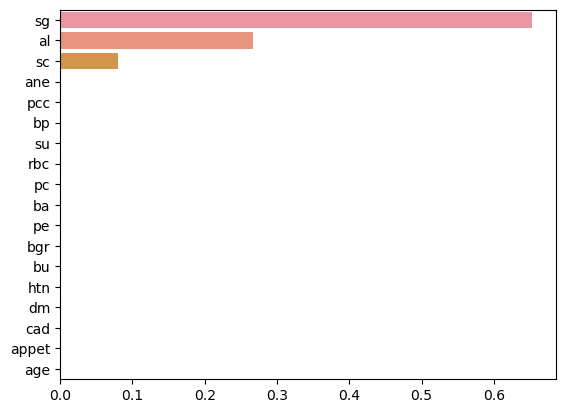
\includegraphics{assignment6111_files/figure-pdf/cell-74-output-1.png}

\begin{itemize}
\tightlist
\item
  We use the max\_depth of \textbf{3} to fit the model. From the plot
  above, we can see that \textbf{sg} has the longest length, which
  indicates the most influence on the output of the model. For those
  features have very short bars represent low importance (they might be
  possible to exclude them from the mode).
\end{itemize}

\begin{enumerate}
\def\labelenumi{\arabic{enumi}.}
\setcounter{enumi}{14}
\tightlist
\item
  Team Contributions:
\end{enumerate}

Junbo Tan: Q1, Q2, Q3, Q7-13 (Decision Tree) Zichuan Xu: Q4, Q5, Q6, Q7
- 12 (Logistic Regression)

\begin{enumerate}
\def\labelenumi{\arabic{enumi}.}
\setcounter{enumi}{15}
\tightlist
\item
\end{enumerate}

\href{\%22https://github.com/Zichuan66/Assignment-6.git\%22}{GitHub
Link}



\end{document}
